\documentclass{article}
\usepackage{amsmath,graphicx,enumerate,hyperref,alltt,theorem}
\usepackage[british]{babel}

%%%%%%%%%% Start TeXmacs macros
\newcommand{\tmem}[1]{{\em #1\/}}
\newcommand{\tmstrong}[1]{\textbf{#1}}
\newcommand{\tmtextbf}[1]{{\bfseries{#1}}}
\newcommand{\tmtextit}[1]{{\itshape{#1}}}
\newenvironment{enumeratealpha}{\begin{enumerate}[a{\textup{)}}] }{\end{enumerate}}
\newenvironment{enumeratenumeric}{\begin{enumerate}[1.] }{\end{enumerate}}
\newenvironment{enumerateroman}{\begin{enumerate}[i.] }{\end{enumerate}}
\newenvironment{itemizearrow}{\begin{itemize} \renewcommand{\labelitemi}{$\rightarrow$}\renewcommand{\labelitemii}{$\rightarrow$}\renewcommand{\labelitemiii}{$\rightarrow$}\renewcommand{\labelitemiv}{$\rightarrow$}}{\end{itemize}}
\newenvironment{itemizedot}{\begin{itemize} \renewcommand{\labelitemi}{$\bullet$}\renewcommand{\labelitemii}{$\bullet$}\renewcommand{\labelitemiii}{$\bullet$}\renewcommand{\labelitemiv}{$\bullet$}}{\end{itemize}}
\newenvironment{itemizeminus}{\begin{itemize} \renewcommand{\labelitemi}{$-$}\renewcommand{\labelitemii}{$-$}\renewcommand{\labelitemiii}{$-$}\renewcommand{\labelitemiv}{$-$}}{\end{itemize}}
\newenvironment{tmindent}{\begin{tmparmod}{1.5em}{0pt}{0pt} }{\end{tmparmod}}
\newenvironment{tmparmod}[3]{\begin{list}{}{\setlength{\topsep}{0pt}\setlength{\leftmargin}{#1}\setlength{\rightmargin}{#2}\setlength{\parindent}{#3}\setlength{\listparindent}{\parindent}\setlength{\itemindent}{\parindent}\setlength{\parsep}{\parskip}} \item[]}{\end{list}}
\newenvironment{tmparsep}[1]{\begingroup\setlength{\parskip}{#1}}{\endgroup}
\newtheorem{definition}{Definition}
{\theorembodyfont{\rmfamily}\newtheorem{example}{Example}}
%%%%%%%%%% End TeXmacs macros

\begin{document}

\title{KeYTestGen2: a verification-driven test case generation
system}
\author{B.Sc. Thesis.\\
\\
\\
}
\maketitle





\begin{abstract}
  Software testing is a common verification technique in software engineering,
  aiding both the development of the system itself, as well as subsequent
  quality assurance, maintenance and extension. It suffers, however, from the
  drawback that writing high quality test cases is an error prone and resource
  heavy process.
  
  
  
  This work describes KeYTestGen2, a verification-driven, automatic test case
  generation system. It addresses the problem of automatically generating \
  robust test code by relying on symbolic execution of Java source code using
  the KeY Symbolic Debugger. This process yields sufficiently detailed data
  about software systems in order to generate tests of high quality.
  KeYTestGen2 implements a robust processing system which can both control
  this process, and mold the generated data into executable test suites for
  modern automated testing frameworks, such as JUnit. 
\end{abstract}



\begin{flushleft}
  \begin{tmparmod}{10cm}{0pt}{0pt}
    \begin{tmparmod}{5cm}{0pt}{0pt}
      \begin{tmparmod}{2cm}{0pt}{0pt}
        \begin{tmparmod}{0pt}{2cm}{0pt}
          {\tmstrong{Acknowledgement}}
          
          
          
          This work has been made possible through the tireless support of the
          KeY community, which has always been available to give me guidance
          in all things related to the project. I especially thank Dr. Reiner
          H{\"a}hnle, Dr. Richard Bubel, Martin Hentschel and their colleagues
          at the Darmstadt University of Technology, for letting me stay and
          work with them leading up to the 2012 KeY Symposium.
          
          
          
          My deepest thanks to Dr. Wolfgang Ahrendt, Gabriele Paganelli and
          the {\tmem{Software Engineering using Formal Methods}} group at
          Chalmers, for inviting me to join them in their work. This project
          would never have started without them.
        \end{tmparmod}
      \end{tmparmod}
    \end{tmparmod}
  \end{tmparmod}
\end{flushleft}





{\pagebreak}

{\tableofcontents}



\section{Introduction}

June 4th, 1996.



It is early afternoon, and despite the unmistakable advance of summer, a
cloud canopy lingers over French Guiana.



The few rays that penetrate the cloud cover proceed to reflect off of the
white-metallic hull of Ariane 5. She towers about 52 metres tall on the launch
pad, her twin boosters already being prepared for her momentous next 5
minutes. She is the latest marvel in European space exploration, the first of
her kind, and has cost over 370 million USD to construct. With her, she
carries 4 Cluster II satellites, which she over the next few hours will deploy
in low orbit in order to help scientists study the interaction between cosmic
rays and the earths magnetic field. \ Expectations from resident ESA officials
could hardly have been higher. Somewhere in the control room, a napkin dries
beads of sweat from the forehead of an operator. Maybe it's the heat.



At 12:33:56 one of the French operators begins to anounce the last 10 seconds
of Arianes time on solid ground. The seconds pass by, the liftoff signal is
given, her boosters flash and shake, and she ascends towards the skies,
carried on a magnificient plume of burning rocket fuel. Her roars can be heard
from kilometres away.



37 seconds later, the burning remains of Ariane 5 are falling back to ground
she left just moments earlier. She has self-destructed in mid launch. Nobody
is injured, but hundreds of millions of invested dollars have been lost in
just a few seconds, and one of the ESA:s most prominent projects has suffered
a catastophic setback. In the control room, more than a few napkins press
against incredulous foreheads. The heat probably has very little to do with it
right now.



Ariane 5 is is dead, because somebody, in the course of her development, had
assumed that it would be safe to round a 64-bit integer to a 16-bit
representation.



It wasn't. \

\subsection{Motivation: the pursuit of correctness}

The Ariane 5 disaster
{\cite{jazequel1997design}}{\cite{dowson1997ariane}}{\cite{lions1996ariane}}
has become a flagship example of the potentially disastrous consequences of
{\tmem{software failure}}. Through her demise, she emphasized the prominence
of one of the great challenges in software engineering: the pursuit of
{\tmem{correctness}} - assuring that a software system functions as intended.



The advent of the Information Age has transformed human civilisation like
nothing else in our history, and we now live in a world which is growing ever
closer to irreversible dependence on computer technology. In modern countries,
computers and the software they run saturate almost every aspect of life, from
keeping the institutions of society running, to helping individuals work and
stay in touch with their loved ones. Due to our dependence on them, we also
deal with the consequences of their failings on an almost daily basis.
Smartphones resetting, laptop screens going black, and word processors
crashing{\footnote{Although, as is commonly known, word processors always wait
to crash until you manage to somehow disable document recovery.}}, are all
symptoms of software failure.



While these examples may be trivial at best, and their consequences
inconvenient at worst{\footnote{Depending on what was in that document you
just lost, of course! }}, the stakes rapidly scale up when we consider just
how many of the more critical elements of our societies depend on software.
Software operates life-support systems, medical instruments{\footnote{In at
least 6 incidents between 1985 and 1987, the Therac-25 radiation therapy
machine delivered massive radiation overdoses to patients, resulting in the
deaths of 5. One of the sources of the malfunction was a race condition in the
control software of the machine.}}, emergency dispatch services, banking
systems, military appliances{\footnote{In 1991, during the Gulf War, a
software failure in a then-deployed Patriot missile battery caused it to fail
to intercept an incoming SCUD ballistic missile, leading to the deaths of 28
soldiers. Scores of others suffered injuries.}}, nuclear reactors, airplanes,
and in important research projects such as the Large Hadron Collider. Here,
our dependence on software means that its cost of failure runs a high risk of
being counted, ultimately, in human lives and property.



With all this in mind, it is clear the pursuit of correctness is one of the
most important tasks in any software engineering process. The present work is
all about contributing to winning that pursuit.



\subsection{Contribution of this work}

This work describes the implementation of {\tmstrong{KeYTestGen2}}, a
{\tmem{verification-driven}}, automatic test case generation system, as well
as the theoretical concepts behind it. It aims to improve the software
engineering process by allowing programmers to easily construct robust and
complete {\tmem{test code}} for their programs.



Below, we elaborate a bit on the importance, strengths and weaknesses of
software testing, and then briefly outline why the contribution of KeYTestGen2
is important in this regard.



\subsubsection{Software testing as a means to correctness}

In contemporary software development, one of the most popular approaches to
verification is {\tmem{software testing}}. Simply put, testing means
constructing a specific starting state (pre-state) for the system, executing
the system (or specific parts of it), and then asserting that the state of the
system after such execution (the post-state) satisfies some specific set of
constraints{\footnote{This notion is formalized in section 2.1.}}.



The wide popularity of testing as a verification approach is based on good
grounds. It is intuitive, generally simple to implement, and enjoys rich tool
support for practically all major programming languages. Such tools frequently
allow the automatic execution of groups of tests, which makes continually
verifying the codebase as it grows an easy task. Finally, testing is also a
flexible approach, which can be applied to several stages of both software
engineering and the system itself.



Testing is no silver bullet in terms of verification, however, and suffers
from two principal drawbacks:
\begin{enumeratenumeric}
  \item Testing is not exhaustive. It can verify that certain specific runs of
  the system behave correctly, but it generally cannot give assurance
  regarding others which it does not cover. To mitigate this, tests can be
  constructed in such a way that they together cover a representative set
  pre-states and execution runs through the source code itself, in order to
  give greater assurance that cases which are not covered may by implication
  work correctly as well.
  
  \item While good tool support exists for it, creating tests can still takes
  considerable time and effort. Further, constructing the kind of high quality
  tests suggested above is generally even more demanding, as it requires
  meticulous investigation of the code itself in order to make sure that all
  relevant inputs and execution paths are covered.
  
  
\end{enumeratenumeric}

\subsubsection{Automated test generation and KeYTestGen2}

One possible way of resolving issue \#2 in the previous section is to
{\tmem{automate}} the test generation process itself. Not only does this take
the burden of writing test code off the programmer, but it can potentially
provide additional, important benefits as well. One such benefit, for example,
would be the possibility to generate test code of a certain {\tmem{quality
level}} which would be difficult for humans to construct manually. A prominent
such criteria is {\tmem{code coverage}}, which we elaborate on in section 2.



\subsubsection{Verification-driven test case generation}

KeYTestGen2 is a verification-driven test case generator, in the sense that it
harvests metadata generated by the proof engine of the KeY
system{\footnote{See section 3.}}. This allows it to thoroughly explore the
possible execution paths through the system under test, select a subset of
them, and then construct test cases for these specific execution paths. By
doing so, KeYTestGen2 effectively addresses the problem of automatically
generating robust test data, as it has the ability to generate tests which
satisfy both code coverage criteria, and potentially various input constraints
as well{\footnote{See section 5.3.3.}}. \

\subsection{Background}

While KeYTestGen2 aims to be novel in its implementation, the concepts it is
based on have been well understood for a long time. Below, we give a brief
overview of {\tmem{KeYTestGen}}, the precursor of KeYTestGen2, and then
explain how KeYTestGen2 improves on this previous work.



\subsubsection{Previous work - KeYTestGen}

As the name implies, KeYTestGen2 is a sequel - although not entirely.



Conceptually, KeYTestGen2 is based on an earlier system called the
{\tmem{Verification-Based Testcase Generator}}, which was developed as part of
research by Dr. Christoph Gladisch, Dr. Bernhard Beckert, and others
{\cite{EngelHaehnle07}}{\cite{Engel2006}}{\cite{BeckertGladisch2007}}{\cite{Gladisch2008_TAP}}{\cite{Gladisch2008}}.
This system was subsequently adopted and further developed by researchers at
Chalmers University of Technology, where it was also (re-)branded as
{\tmem{KeYTestGen}} {\cite{Paganelli2010}}.



The idea behind KeYTestGen was to create a glass box test generation
system{\footnote{See section 2.7.3.}} based on the state-of-the-art symbolic
execution{\footnote{See section 3.2.}} system used in KeY
{\cite{EngelHaehnle07}}. The symbolic execution carried out by KeY, due to its
rigour{\footnote{A virtue of KeY being a deductive verification tool.}},
explored the source code of Java programs so thoroughly that the resulting
metadata could be used to create test cases satisfying such rigorous code
coverage criteria as MC/DC{\footnote{See section 2.5.2.}}.



KeYTestGen showed itself to be a powerful proof of concept, being used by
Chalmers in at least one international research project, and even recieving
mention by the ACM. For various reasons, \ however, the developers behind it
abandoned the project, and it is currently no longer being actively
maintained{\footnote{While the source code of KeYTestGen is no longer being
distributed as part of the mainline KeY system, it still exists on a separate
development branch. An executable legacy version of the system itself is still
available for download on the KeY homepage.}}.



\subsubsection{Towards KeYTestGen2}

Despite its name, KeYTestGen2 is not an attempt to resurrect KeYTestGen.
Rather, it is an attempt to create, completely from scratch, a novel white box
test case generation system based on the same fundamental principles as the
original KeYTestGen. It is designed to provide the same basic functionality as
its predecessor, while at the same time bringing a host of new features to the
table. Ultimately, KeYTestGen2 is aimed to be useful in an actual, industrial
context.



\subsubsection{Target platforms}

KeYTestGen2 is purely implemented in Java, and can hence execute on all
platforms capable of running a Java Virtual Machine. As input, it consumes
Java source files.



The system produces output in a variety of formats, including XML and
JUnit{\footnote{See section 2.4.1.}}, the latter being our focus of attention
in this work.

\subsection{Organization of this work}

The remainder of this work is broken up into 5 sections:
\begin{itemizedot}
  \item {\tmstrong{Section 2}} is an introduction to the general theoretical
  concepts behind KeYTestGen2. Here we introduce software verification,
  testing, symbolic execution, and related concepts. This section is provided
  for the sake of context, and readers familiar with these concepts can ignore
  it, or refer to select parts.
  
  \item {\tmstrong{Section 3 }}provides an introduction to the KeY system, the
  parent project of KeYTestGen2, which also forms its technological
  foundation.
  
  \item {\tmstrong{Section 4}} describes the architecture and implementation
  of KeYTestGen2 itself.
  
  \item {\tmstrong{Section 5}} gives an evaluation of the work done thus far,
  outlines ongoing work, and discusses future plans for the project.
  
  \item {\tmstrong{Section 6}} gives a conclusion to the work.
\end{itemizedot}
\section{Fundamental concepts}

In this section, we will lay a theoretical foundation for the rest of the work
by outlining the central concepts underpinning its functionality.



We will begin by looking at software verification and verification methods,
focusing especially on {\tmem{software testing}} as a verification method.
Here, we formally define concepts central to testing itself, as well as the
related testing quality metric known as {\tmem{code coverage}}.



Following this, we cover {\tmem{test automation}} - first the automation of
the test execution process, and then the central interest of this work:
automating the test case generation process itself. Here, we introduce black
box and white box test generation systems, focusing on the white box ones, in
connection with which we also introduce the conept of {\tmem{symbolic
execution}}.

\subsection{Specifications - formalizing correctness}

Until now we have been content with using a rather loose definition of
correctness, simply saying that software should ``function as intended''.
Here, we will formalize this notion of correctness. To do so, we need to
introduce the notion of a {\tmem{specification}}.



\begin{tmparmod}{1cm}{0pt}{0pt}
  \begin{tmparmod}{0pt}{1cm}{0pt}
    {\noindent}{\noindent}\begin{tabular}{l}
      \begin{definition}
        
        
        
        
        A \tmtextbf{specification} for some code segment \tmtextbf{m} in some
        software system \tmtextbf{s} is a triple
        
        \ \
        
        \ \ \ \ \ \ \ (Pre, m, Post)
        
        
        
        where Pre (or \tmtextbf{preconditions}) is a set of constraints on the
        state of \tmtextbf{s} immediately prior to the execution of
        \tmtextbf{m}, and Post (\tmtextbf{postconditions}) is a set of
        constraints on the state of \tmtextbf{s} immediately after the
        execution of \tmtextbf{m} terminates, s.t. Pre -> Post (Post always
        holds given that Pre holds).
        
        
        
        By ``state of s'' we mean both the internal state of s itself, as well
        as any external factors which s depends on, such as a database,
        sensor, etc. {\tmem{}} 
      \end{definition}
    \end{tabular}{\hspace*{\fill}}{\smallskip}
  \end{tmparmod}
\end{tmparmod}





Specifications are also commonly called {\tmem{contracts}}, since they specify
a contractual relationship between software and the entity invoking it (the
{\tmem{callee}} and {\tmem{caller}}). Under this contract, the callee gives
certain guarantees (i.e. the postconditions) to the caller, given that the
caller satisfies certain criteria (the preconditions) regarding how the call
is made. \



\subsubsection{The Java Modelling Language}

In Java, specifications can be expressed informally as part of Javadoc
comments{\footnote{It should be noted that the JavaDoc specification has
native tags for expressing specifications, such as @pre and @inv. These are
nowhere near expressive enough to write thorough specifications, however.}} or
ordinary comments. However, a more rigorous approach is to use a
\tmtextit{specification language}. These are languages developed specifically
for formulating rigorous and non-ambigous specifications for software.



For Java, perhaps the most prominent such language is the Java Modelling
Language; JML {\cite{JMLwebsite}}{\cite{JML-Ref-Manual}}. JML is written
inside ordinary Java comments for the code it relates to.



\begin{tmparmod}{1cm}{0pt}{0pt}
  \begin{tmparmod}{0pt}{1cm}{0pt}
    {\noindent}{\noindent}\begin{tabular}{l}
      \begin{example}
        A formally specified Java method.
        
        
        
        The following is a specification for a simple addition function for
        positive intergers. The specification is expressed in the JML
        language.
        
        
        
        \begin{tmparmod}{1cm}{0pt}{0pt}
          /*@ public spec normal\_behavior
          
          \ @ requires x > 0 \& y > 0
          
          \ @ ensures {\textbackslash}result == x + y \ \&
          {\textbackslash}result \ > 0
          
          \ @*/
          
          public static void addWholePositive(int x, int y)\{
          
          \ \
          
          \ \ if(x < 0 || y < 0) \{
          
          \ \ \ \ \ throw new
          
          \ \ \ \ \ \ \ \ IllegalArgumentException(
          
          \ \ \ \ \ \ \ \ \ \ \ \ "Not a positive whole number");
          
          \ \ \}
          
          
          
          \ \ return x + y;
          
          \}
        \end{tmparmod}
        
        
        
        The \tmtextbf{requires} clause here contain the preconditions, while
        the \tmtextbf{ensures} clause contains the postconditions.
        {\textbackslash}result denotes the value returned by the function. As
        can be easily seen here, this specification guarantees that the result
        will equal x+y and be greater than 0, if parameters x and y are both
        greater than 0 at the time of invocation.
      \end{example}
    \end{tabular}{\hspace*{\fill}}{\smallskip}
  \end{tmparmod}
\end{tmparmod}

\subsection{Software verification and verification methods}

\ In software development, the process of ensuring the correctness of
software is called {\tmem{verification}}{\footnote{Verification is a rich
field of research and application all by itself, and we will only skim the
surface here in order to create context for the rest of this work.}}. A given
approach to verifying software is called a {\tmem{verification method}}.



\subsubsection{The verification ecosystem}

Today, there is a wide array of verification methods available. To get an
overview of the ecosystem they make up, we may classify{\footnote{In addition
to what is described here, methods are commonly grouped in terms of whether
they are {\tmem{static}} or {\tmem{dynamic}}. Static methods verify code
without actually executing it, and includes both informal methods such as code
inspection and tool-supported introspection, and formal methods such as model
checking. Dynamic methods rely on observing the system under execution, and
include informal approaches like testing, and more formal ones like runtime
monitors. We do not distinguish between these categories here, as there is no
need to understand it in order to understand KeYTestGen2 or its concepts.}}
them according to the {\tmem{degree}} {\tmem{}}of correctness they are
intended to provide. We can think of them as spread across a spectrum, ranging
from methods that take a rather lightweight and informal approach, to methods
which are much more rigorous and approach mathematical precision in the kind
of correctness they guarantee.



\subsubsection{The formal methods} \

On the rigourous end of this spectrum we find the {\tmem{formal methods}},
which take a strict approach to correctness, generally requiring a
mathematical or otherwise exhaustive demonstration that the software conforms
to its specification.



One prominent example of this approach is {\tmem{deductive verification}},
which treats the actual program code and its specification as part of some
kind of logic, and uses a calculus for the same logic to deduce whether or not
the code is correct with regard to the specification. The KeY system, which we
will examine later, follows this approach.

Another widely used approach is {\tmem{model checking}}, which relies on
constructing a model of the system, and then verifying properties of this
model. If the properties can be shown to hold for the model, it (usually)
follow that they hold for the software itself.



The chief strength of formal methods is precisely their more complete approach
to correctness: if a logical proof, validated model or equivalent can be
obtained for some behavior of the software, we can be reasonably
assured{\footnote{We can never be completely assured of this, as formal
methods often only work on the source code level of the software itself. To
assure 100\% correctness, we would need to formally verify any underlying
implementations as well, including compilers, interpreters, VMs and operating
systems. Such extensive formal verification is usually infeasible.}} that this
behavior will always hold during runtime. For safety-critical applications,
such as aircraft control systems, formal methods is often the desired approach
to verification due to their demand for, practically, totally fail-safe
operation.



On the downside, formal verification is usually a resource heavy process,
requiring special tool support, specialist training, and planning in order to
be effectively deployed, or even feasible at all. Applying it to larger, or
even general projects which do not require such a strict degree of correctness
may thus not be a viable option.



\subsubsection{Software testing}

On the other end, we find the various, informal {\tmem{testing methods}}. The
basic idea behind these is executing the system - in whole or in part - with
some well-defined input and subsequently analyzing the output of the
execution, usually by comparing it to some expected output. Just what such
expected output and well-defined input should be, is usually determined
(respectively) by analyzing the postconditions and preconditions for the parts
being tested.



Testing methods benefit from being (much!) more intuitive and easy to use, as
they embody what programmers normally do to check their code: specify some
controlled input, execute the code, and determine if the output conforms to
expected behavior. Due to this, testing is generally easier to adopt and use,
as compared to the formal methods. The fundamental simplicity of testing also
makes it a highly flexible process which easily scales to a wide range of
applications.



The simplistic and informal nature of testing, however, is also its chief
weakness. Since testing is not exhaustive{\footnote{We can of course make
testing exhaustive by constructing tests for {\tmem{all}} possible ways a
system can perform a given task. However, it is obvious that this does not
scale even for trivial programs. Furthermore, if we are looking for
verification by exhaustive examination of possible executions, this is exactly
what model checking is}}, its degree of guaranteed correctness is far less
than that of formal methods. As Edsgar Dijkstra put it,

\begin{quote}
  {\tmem{``testing can demonstrate the presence of errors, but never their
  absence''}}
\end{quote}

In other words, testing a system can helps us to locate bugs in it, but unlike
a formal proof it can never give us any broader guarantees about the system
actually being correct with regards to its specification.



In terms of time and resources invested, testing is not always necessarily
cheap, either. Writing test cases is an engineering discipline in its own
right, and depending on the target extent of testing for a given system, it
can in severe cases take more time to write tests for the system than the
system itself.

Further, since the quality of a set of tests very much depend on how well it
explores interesting execution paths in the system under test, considerable
care has to be taken in order to avoid gaps in such coverage. All of this
takes time, and in many cases, like with the formal methods, special training
of team members responsible for testing. It is also very easy, despite all
this, to get it wrong.



Despite its problems, the simplicity and flexibility of testing still makes
it one of the most frequently used verification methods in the contemporary
industry, enjoying a broad range of tool support and studies. In the present
work, this is the manner of verification we will put the brunt of our focus
on.

\subsection{Unit testing}

Testing can be done at several levels of granularity, ranging from testing the
complete system, to testing interaction between modules, down to testing only
atomic {\tmem{units}} of functionality {\cite{SoftwareEngineering9}}. In most
programming languages, such units correspond to a function or routine (or
method in an object oriented context). Testing such units is predictably
called {\tmem{unit testing}}.



A {\tmem{test case}} represents a single test for some unit in a software
system. Formally, we define it like this:



\begin{tmparmod}{1cm}{0pt}{0pt}
  \begin{tmparmod}{0pt}{1cm}{0pt}
    {\noindent}{\noindent}\begin{tabular}{l}
      \begin{definition}
        
        
        
        
        Given a unit {\tmem{{\tmstrong{u}}}}, a \tmtextbf{test case}
        {\tmem{{\tmstrong{T}} }}for {\tmem{u}} is a tuple
        ({\tmstrong{{\tmem{In}}}}, {\tmem{{\tmstrong{Or}}}}), where
        \begin{itemize}
          \item In (``input'') is a tuple ({\tmem{{\tmstrong{P}}}},
          {\tmstrong{{\tmem{S}}}}), where
          \begin{itemizeminus}
            \item P is a set of parameter values to be passed to {\tmem{u}},
            and
            
            \item S is the state of the surrounding system as {\tmem{u}}
            starts executing.
          \end{itemizeminus}
          \item Or (``oracle'') is a function
          Or({\tmem{}}{\tmem{{\tmstrong{R{\tmstrong{}}}}}},
          {\tmem{{\tmstrong{F}}}}) -> \{true, false\}, where
          \begin{itemizeminus}
            \item R is the return value of {\tmem{u}} (if any), and
            
            \item F is the state of the system after {\tmem{u}} terminates.
          \end{itemizeminus}
          Or returns {\tmstrong{{\tmem{true}}}} if R and F match the expected
          system state after the unit terminates, and
          {\tmstrong{{\tmem{false}}}} otherwise. 
        \end{itemize}
      \end{definition}
    \end{tabular}{\hspace*{\fill}}{\smallskip}
  \end{tmparmod}
\end{tmparmod}





The common approach in contemporary practice is to organize test cases into
{\tmem{test suites}}, where each such test suite consists only of test cases
for a given method. While other such organizations exist, this is the approach
followed by KeYTestGen2.



\begin{tmparmod}{1m}{0pt}{0pt}
  \begin{tmparmod}{1cm}{0pt}{0pt}
    \begin{tmparmod}{0pt}{1cm}{0pt}
      {\noindent}{\noindent}\begin{tabular}{l}
        \begin{definition}
          
          
          
          
          Given a unit {\tmem{{\tmstrong{u}}}} and a set of test cases
          {\tmstrong{{\tmem{Ts}}}} for {\tmem{u}}, the tuple (u, Ts) is
          referred to as a {\tmstrong{test suite}} for {\tmem{u}} .
        \end{definition}
      \end{tabular}{\hspace*{\fill}}{\smallskip}
    \end{tmparmod}
  \end{tmparmod}
\end{tmparmod}





Unit testing is a desirable level of granularity for many reasons. In
particular, it can be used from the very beginning in most software
engineering processes, since it requires only that the system contains a
single unit to start writing tests for{\footnote{In fact, there are software
engineering processes which are completely test-driven, and advocate writing
the tests {\tmem{before}} the actual code is even implemented. A prominent
example of such a process is {\tmem{Test-Driven Development}}.}}. Further,
unit testing is useful in debugging, as the cause for a test failing can be
tracked down to a single unit and tackled there. This makes it an excellent
tool for isolating regressions in the code as it is being developed and
extended.



The remainder of this work assumes we are working in a unit testing
environment, and this is the granularity we will have in mind whenever we
mention testing for the remainder of it.

\subsection{Test frameworks}

A larger system will usually consist of hundreds - if not thousands - of
individual units. Assuming we wish to create at least one test case for each
of the non-trivial ones{\footnote{i.e. setters, getters and the like.}} (which
is usually the case), we will swiftly end up with a massive pool of test code
to manage. In addition to that, we still need some kind of tool or scripting
support for effectively executing the test cases, tracking down failures, and
so forth.



The definitive way to make this easy is to use a {\tmem{test framework}} for
developing and running our unit tests. Such a framework will usually contain
both a toolkit for developing and structuring the test cases themselves, as
well as a comprehensive environment to run and study their output in. Today,
at least one such framework exists for practically every major programming
language in existence.



\subsubsection{xUnit}

The most popular family of unit testing frameworks in contemporary use is
most likely xUnit. Initially described in a landmark paper by Kent Beck
{\cite{Beck1989}} on testing SmallTalk code, xUnit is now implemented for a
wide range of programming languages{\footnote{For Java, the language which we
are concerned with here, the most popular such implementation is called
JUnit.}}.



In an xUnit framework, a set of xUnit tests are created for a subset of the
units in the system to be tested. Each such test generally has the following
life cycle {\cite{TestPatterns2007}}:
\begin{enumeratenumeric}
  \item \tmtextit{Setup} a \tmtextit{test fixture}. Here, we set up everything
  that has to be in place in order for the test to run as intended. This
  includes instantiating the system as a whole to a desired state, as well as
  creating any necessary parameter values for the unit. \
  
  \item \tmtextit{Exercise} the test code. Here, we execute the unit itself
  with the parameters generated above, starting in the system state generated
  above.
  
  \item \tmtextit{Verify} the system state after the unit finishes executing.
  Here, we use a \tmtextit{test oracle} - a boolean function, to evaluate if
  the resulting state of the system satisfies our expectations. For example,
  for a method pushing an object to a stack, the oracle might verify that the
  stack has been incremented, and that the object on top is the object we
  expected to be pushed. \
  
  \item \tmtextit{Tear down} the test environment. Here, we undo whatever the
  previous 3 steps did to the system state, restoring it to a mint condition
  ready to accept another test case.
\end{enumeratenumeric}

\subsection{Coverage criteria - a metric for test quality}

We have now introduced how to construct and organize test cases, but we still
have not said much about how we can determine their {\tmem{quality}} with
regard to the code they are testing. Since we are dealing with the correctness
of software, having a metric for measuring this is of course desirable.



One metric we can use is to measure the degree to which test cases
{\tmem{cover}} various aspects of the unit they are written for. Such coverage
can cover several things, for example the range of inputs for the unit, or the
execution of the statements in the source code of the unit itself. The former
is known as {\tmem{input space coverage}}, the latter as {\tmem{code
coverage}} {\cite{ammann2008introduction}}. It is the latter that is our prime
concern in this work.



To see why code coverage is important, let's consider an example:



\begin{tmparmod}{1cm}{0pt}{0pt}
  \begin{tmparmod}{0pt}{1cm}{0pt}
    {\noindent}{\noindent}\begin{tabular}{l}
      \begin{tmparmod}{1cm}{0pt}{0pt}
        \begin{example}
          
        \end{example}
        
        Consider the function:
        
        
        
        \ \ int processBranch(int num) \{
        
        \ \ \ \ \ switch(num) \{
        
        \ \ \ \ \ \ \ \ case 1: return processOne();
        
        \ \ \ \ \ \ \ \ case 2: return processTwo();
        
        \ \ \ \ \ \ \ \ case 3: return processThree();
        
        \ \ \ \ \ \}
        
        \ \ \}
        
        
        
        We construct the following test suite with some unspecified oracle:
        
        \tmtextit{ \ T1: }(1, \tmtextit{oracle})
        
        \tmtextit{ \ T2: }(3, \tmtextit{oracle}) 
      \end{tmparmod}
      
      
    \end{tabular}{\hspace*{\fill}}{\smallskip}
  \end{tmparmod}
\end{tmparmod}





Under this test suite, the switch-branch triggered when num is 2 will never be
taken. To see why this is a serious problem, we need only consider situtations
where processTwo() throws an exception, has undesirable side effects, or
otherwise functions improperly with regard to the input for the unit. This
will {\tmem{not}} be uncovered if we rely only on the test cases provided - we
hence say that we {\tmem{lack code coverage}} for the execution path(s)
leading to processTwo(). For our test suite to be genuinely robust, we would
need to introduce at least one more test case which would cause processTwo()
to be executed as well.



Code coverage is not a monolithic concept, and there exist a great deal of
different {\tmem{code coverage criteria}} defining defining different degrees
of code coverage. We will describe some of the most prominent of these
criteria for the purpose of our work here. They can generally be divided into
two categories - {\tmem{logic coverage}} and



\subsubsection{Graph coverage}

Graph coverage critera are defined based on a \tmtextit{control flow graph}
representation of the unit under test. Such a graph is effectively an
abstraction showing the different execution paths which may be taken through
the code of the unit itself.



\begin{tmparmod}{1cm}{0pt}{0pt}
  \begin{tmparmod}{0pt}{1cm}{0pt}
    {\noindent}{\noindent}\begin{tabular}{l}
      \begin{definition}
        
        
        
        
        A \tmtextbf{control flow graph} is a directed, possibly cyclic graph
        where:
        \begin{itemizedot}
          \item nodes are program statements,
          
          \item edges are transitions between such statements, and
          
          \item each such edge may have a \tmtextbf{transition condition},
          which is a boolean decision that must hold in the first node of the
          edge, in order for the transition to the second node to be taken.
        \end{itemizedot}
      \end{definition}
      
      Such a graph has:
      \begin{itemizedot}
        \item exactly one entry point, and
        
        \item one or more exit points, corresponding to invocation and return
        statements in the code being thus represented.
      \end{itemizedot}
      
    \end{tabular}{\hspace*{\fill}}{\smallskip}
  \end{tmparmod}
\end{tmparmod}





Since such a graph represents an executable piece of code, we also define the
concepts of an {\tmem{execution path}} and {\tmem{path condition}} wrt. to it.





\begin{tmparmod}{1cm}{0pt}{0pt}
  \begin{tmparmod}{0pt}{1cm}{0pt}
    {\noindent}{\noindent}\begin{tabular}{l}
      \begin{definition}
        
        
        
        
        Given a control flow graph {\tmem{{\tmstrong{G{\tmstrong{}}}}}}, an
        {\tmstrong{execution path}} {\tmstrong{{\tmem{EP{\tmstrong{}}}}}} is a
        path through G, s.t. EP begins at the entry point of G, and ends at
        exactly one of the exit points of G. 
      \end{definition}
    \end{tabular}{\hspace*{\fill}}{\smallskip}
  \end{tmparmod}
\end{tmparmod}





\begin{tmparmod}{1cm}{0pt}{0pt}
  \begin{tmparmod}{0pt}{1cm}{0pt}
    {\noindent}{\noindent}\begin{tabular}{l}
      \begin{definition}
        
        
        
        
        Given a control flow graph {\tmem{{\tmstrong{G{\tmstrong{}}}}}} and an
        execution path{\tmstrong{ {\tmem{EP{\tmstrong{}}}}}}, a
        {\tmstrong{path condition}} {\tmem{{\tmstrong{PC}}}}, is a boolean
        constraint which, if it holds when the graph is entered, causes EP to
        be taken through the graph.
      \end{definition}
    \end{tabular}{\hspace*{\fill}}{\smallskip}
  \end{tmparmod}
\end{tmparmod}





In this context, given that we have a some unit represented by a control flow
graph, a test suite can satisfy the criteria listed below{\footnote{We only
provide a formal definition for the first one, as the other two are defined in
the same way by exchanging `''statement'' for `edge'' and ``execution path'',
respectively.}}:
\begin{itemizedot}
  \item {\tmstrong{Statement coverage}} - all statements in the unit are
  executed at least once.
  
  \item {\tmstrong{Branch coverage}} - all possible transitions between two
  adjacent statements are taken at least once.
  
  \item {\tmstrong{Path coverage}} - each possible execution path for the unit
  is taken at least once.
\end{itemizedot}


\begin{tmparmod}{1cm}{0pt}{0pt}
  \begin{tmparmod}{0pt}{1cm}{0pt}
    {\noindent}{\noindent}\begin{tabular}{l}
      \begin{definition}
        Statement coverage
        
        
        
        Given a control flow graph {\tmem{{\tmstrong{G{\tmstrong{}}}}}} and a
        test suite {\tmem{{\tmstrong{TS}}{\tmstrong{}}}}, TS satisfies
        {\tmstrong{statement coverage}} wrt. G, iff. for each node
        {\tmstrong{{\tmem{n}}}} in G, there exists a test case {\tmstrong{t}}
        in TS s.t. t causes an execution path through G via n. 
      \end{definition}
    \end{tabular}{\hspace*{\fill}}{\smallskip}
  \end{tmparmod}
\end{tmparmod}

\begin{tmparmod}{1cm}{0pt}{0pt}
  \begin{tmparmod}{0pt}{1cm}{0pt}
    
  \end{tmparmod}
\end{tmparmod}



In terms of quality, each criteria above, in order of definition, effectively
subsumes the ones before it and is hence more robust than they
are{\footnote{In reality, the last criteria, path coverage, is effectively
impossible or infeasible to achieve for non-trivial code, since the presence
of loop statements will cause a combinatiorial explosion in terms of possible
execution paths. }}.



While graph coverage give good coverage with regard to the {\tmem{structure}}
of the code being tested, they tell us relatively little about the more
detailed aspects of the code, such as branch conditions. To reach the kind of
coverage level commonly employed in actual industry, we need to introduce the
class of {\tmem{logic coverage}} criteria.



\subsubsection{Logic coverage}

Logic coverage criteria are defined with regard to boolean {\tmem{conditions}}
and {\tmem{decisions}} present in the code under test.



\begin{tmparmod}{1cm}{0pt}{0pt}
  \begin{tmparmod}{0pt}{1cm}{0pt}
    {\noindent}{\noindent}\begin{tabular}{l}
      \begin{definition}
        
        
        
        
        A \tmtextbf{condition} is an atomic boolean expression, i.e. it cannot
        be sub-divided into further boolean expressions.
        
        
        
        In many contemporary languages, examples of such include
        \begin{itemizedot}
          \item the comparators (<, <=, >, >=)
          
          \item the comparators (!=, ==), iff. the operands of either are
          non-boolean types.
          
          \item boolean literals (true, false)
          
          \item boolean variables and
          
          \item boolean functions.
        \end{itemizedot}
      \end{definition}
    \end{tabular}{\hspace*{\fill}}{\smallskip}
  \end{tmparmod}
\end{tmparmod}





\begin{flushleft}
  \begin{tmparmod}{1cm}{0pt}{0pt}
    \begin{tmparmod}{0pt}{1cm}{0pt}
      {\noindent}{\noindent}\begin{tabular}{l}
        \begin{definition}
          
          
          
          
          Let {\tmem{{\tmstrong{x}}{\tmstrong{}}}} be an arbitrary condition,
          and let {\tmstrong{!}}, {\tmstrong{\&\&}}, {\tmstrong{||}},
          {\tmstrong{==}}, and {\tmstrong{!=}} be the boolean operators NOT,
          AND, OR, EQUALS and NOT-EQUALS (respectively). A boolean
          {\tmstrong{expression}} {\tmem{{\tmstrong{e}}}} is then defined as
          follows:
          
          
          
          d ::= x
          
          d ::= (d)
          
          d ::= !d
          
          d ::= d || d
          
          d ::= d \&\& d
          
          d ::= d == d
          
          d ::= d != d
          
          
          
          A {\tmstrong{decision}} {\tmstrong{{\tmem{d}}}} in some program
          {\tmem{{\tmstrong{p}}}} is an expression whose outcome will cause a
          branching in the execution of p.
        \end{definition}
      \end{tabular}{\hspace*{\fill}}{\smallskip}
    \end{tmparmod}
  \end{tmparmod}
\end{flushleft}





\begin{tmparmod}{1cm}{0pt}{0pt}
  \begin{tmparmod}{0pt}{1cm}{0pt}
    {\noindent}{\noindent}\begin{tabular}{l}
      \begin{example}
        
        
        
        
        Given the following Java code: \
        
        {\noindent}\begin{tmindent}
          \begin{tmparsep}{0em}
            if(a \&\& b || !a \&\& (x<y)) \{
            
            \ \ \ doSomething();
            
            \} else \{
            
            \ \ \ doSomethingElse();
            
            \}
          \end{tmparsep}
        \end{tmindent}{\hspace*{\fill}}{\medskip}
        
        The following is a decision: a \&\& b || !a \&\& (x<y)
        
        
        
        Analysing its composition, we identify the following conditions:
        \begin{itemizeminus}
          \begin{itemizedot}
            \item Boolean variables \tmtextbf{a} and \tmtextbf{b}
            
            \item Comparison x<y, where x and y are comparable (non-boolean)
            values.
            
            \item The negation !a
          \end{itemizedot}
        \end{itemizeminus}
        
        
        An important observation to make here, is that a and !a are
        \tmtextbf{separate} conditions, even though they both contain the same
        boolean variable a.
      \end{example}
    \end{tabular}{\hspace*{\fill}}{\smallskip}
  \end{tmparmod}
\end{tmparmod}





In this context, we define the following basic logic coverage criteria:
\begin{itemizedot}
  \item {\tmstrong{Condition coverage}} - each condition in the code will
  evaluate at least once to true, and at least once to false.
  
  \item {\tmstrong{Decision coverage }}- each decision in the code will
  evaluate at least once to true, and at least to false.
\end{itemizedot}


\begin{tmparmod}{1cm}{0pt}{0pt}
  \begin{tmparmod}{0pt}{1cm}{0pt}
    {\noindent}{\noindent}\begin{tabular}{l}
      \begin{definition}
        Condition coverage
        
        
        
        Given a program {\tmem{{\tmstrong{P{\tmstrong{}}}}}} and a test suite
        {\tmem{{\tmstrong{TS}}{\tmstrong{}}}}, TS satisfies
        {\tmstrong{condition coverage}} wrt. P, iff. for each non-constant
        condition {\tmem{{\tmstrong{c}}}}, s.t. c is part of a decision in P,
        there exists a test case {\tmem{{\tmstrong{t1}}}} and a test case
        {\tmem{{\tmstrong{t2}}}} in TS s.t. t1 causes c to become false, and
        t2 causes it to become true. 
      \end{definition}
    \end{tabular}{\hspace*{\fill}}{\smallskip}
  \end{tmparmod}
\end{tmparmod}





While these are fundamental in terms of logic coverage, we now define a more
advanced criteria which is of special interest to us, because it plays a
prominent role in industrial software verification{\footnote{MC/DC is required
by the Avionics Cerification Standard DO-178B in order to verify software
graded as Level A, i.e. software whose failure is deemed ``catastrophic''
(such as control software for aircraft).}}: the {\tmem{modified condition /
decision coverage}} criterion, or {\tmem{MC/DC}}
{\cite{hayhurst2001practical}}{\cite{chilenski2001investigation}}.





\begin{tmparmod}{1cm}{0pt}{0pt}
  \begin{tmparmod}{0pt}{1cm}{0pt}
    {\noindent}{\noindent}\begin{tabular}{l}
      \begin{definition}
        MC/DC
        
        
        
        Given a program {\tmem{{\tmstrong{P{\tmstrong{}}}}}} and a test suite
        {\tmem{{\tmstrong{TS}}{\tmstrong{}}}}, TS satisfies
        {\tmstrong{Modified Condition / Decision Coverage}} wrt. P, iff.
        
        
        \begin{enumeratenumeric}
          \item TS satisfies Statement Coverage for P,
          
          \item TS satisfies Condition Coverage for P,
          
          \item TS satisfies Decision Coverage for P,
          
          \item Every point of entrance to the program has been executed at
          least once,
          
          \item Every point point of exit from the program has been executed
          at least once,
          
          \item For each condition {\tmem{{\tmstrong{c}}}} in each decision
          {\tmem{{\tmstrong{d}}}} in P, c is shown to independently affect the
          outcome of d.
          \begin{enumerateroman}
            \item I.e. given that all other conditions in d are held fixed,
            changing the value of c alone is shown to affect what d evaluates
            to. 
          \end{enumerateroman}
        \end{enumeratenumeric}
      \end{definition}
    \end{tabular}{\hspace*{\fill}}{\smallskip}
  \end{tmparmod}
\end{tmparmod}







While being an extremely robust criteria, MC/DC is also notoriously difficult
to satisfy (if it can be satisfied at all), due to the sheer number of demands
it puts on the resulting test suite. Depending on how the code under test is
structured, a test suite satisfying MC/DC may further be very large in terms
of the number of test cases it contains.



\subsubsection{Code coverage and automatic test case generators}

The very nature of code coverage makes it practically impossible for black box
test generators to guarantee it. The natural approach to guaranteeing code
coverage is the use of a white box or hybrid system.

\subsection{Automating testing}

One of the great benefits usually offered most test frameworks is the ability
to {\tmem{automate}} large amounts of the testing process, especially the
setting up of test environments and the execution of the tests themselves. The
programmer can thus devote herself entirely to writing test suites, and then
simply hand these over to the frameworks execution system for automatic runs,
saving a lot of time and effort. It also means that the tests can easily be
re-run without much efforts, which makes regression testing when refactoring
or extending the system very easy, as the tests can simply be re-run
repeatedly to verify that modifications to the system don't cause existing
test suites to fail.

\subsection{Automating test case generation}

While test frameworks can help in automating the {\tmem{execution}} of test
cases, they do not readily address the more expensive problem of
{\tmem{creating}} them.



One attempt to overcome this hurdle is the use of {\tmem{test case generation
systems}}. Such systems will usually consume a portion of source code along
with some metadata about it (such as its specification), and attempt to
generate a set of tests for it based on this information.



Depending on how they approach test case generation, we can broadly classify
such systems into two primary categories: black-box and white-box generators.
There is also a hybrid category, referred to as glass box{\footnote{Or ``grey
box''.}} generators.



\subsubsection{Black box test generators}

Black box test generators do their work based on metadata {\tmem{about}} the
unit being tested. For example, given some unit with an associated
specification, a black box generator can analyze the preconditions for the
unit in order to generate a set of test fixtures, and the postconditions in
order to generate a corresponding set of oracles. Each such fixture-oracle
pair is then encoded as a single test case. A system taking this approach is
JMLUnitNG {\cite{JMLUnitNGWebsite}}.



\subsubsection{White box test generators}

Unlike their black box counterparts, white box test case generators can use
the actual implementation code of the unit being tested in order to produce
their output. As such, they are able explore the actual implementation of the
unit in order to gather information about it, allowing for the generation of
more surgical test cases. For example, a white box generator could determine
the exact input needed for a certain exception to be raised, or for a certain
set of statements to be executed, and generate a test case accordingly.



\subsubsection{Glass box test generators}

Glass box systems are hybrid systems, using both metadata about the
implementation as well as the implementation itself in order to generate test
cases. As such, they subsume the functionality of both In practice, this means
that they are able to generate much more expressive and robust test cases than
either of the others.



How the source code is explored can vary widely between implementations.
KeYTestGen2, which falls into this category of generators, uses a method known
as {\tmem{symbolic execution}}, which we will explore in section 3.

\section{The KeY system}

In this section, we introduce the technological foundation for KeYTestGen2
itself, which is KeY system and its Symbolic Debugger. The aspect of KeY of
greatest interest to us is its {\tmem{symbolic execution}} engine, and we will
give an abstract view of how this process works{\footnote{For a full treatise
of how KeY works, please see {\cite{KeYBook2007}}. Here, we will merely cover
enough to discuss the implementation of KeYTestGen2 in the following
section.}}. After this, we will briefly introduce the Symbolic Debugger, which
encapsulates this process on behalf of KeYTestGen2.

\subsection{KeY - an overview}

KeY
{\cite{KeY2005}}{\cite{KeYBook2007}}{\cite{AhrendtEtAl2007}}{\cite{KeYwebsite}}
is a system for integrated, deductive software design, specification,
implementation and verification, jointly developed by several European
universities{\footnote{Currently Chalmers University of Technology, Sweden,
Darmstadt University of Technology and Karlsruhe Institute of Technology,
Germany.}}. It aims to be a novel, powerful formal verification system
applicable to a wide range of industrial software engineering contexts.



KeY takes a {\tmem{deductive}} approach to verification, and attempts to
construct a logical proof that the preconditions of the verified system imply
its postconditions, based on the structure of the code itself. It does so by
translating both the code and its specification into a {\tmem{dynamic logic}}
called JavaDL {\cite{BeckertKlebanov2007}}, creating a {\tmem{proof
obligation}} - a logical proposition which will have to be proved in order to
conclude that the specification is respected by the code. This proof process
is carried out through the use of a semi-automatic theorem prover.

\subsection{Symbolic Execution}

A core aspect of the proof process of KeY is {\tmem{symbolic execution}}. When
KeY attempts to prove a precondition-postcondition implication, it does so by
symbolically ``executing'' each succesive Java statement in the code, encoding
its effects on the overall program state.



Whenever this process encounters a statement which may have several different
outcomes, such as an if-statement, the proof process will have to
{\tmem{branch}}, effectively creating several new proof obligations for each
branch created. As such, over time, the symbolic execution process constructs
a {\tmem{symbolic execution tree}}. An example is given below.



\begin{tmparmod}{1cm}{0pt}{0pt}
  \begin{tmparmod}{0pt}{1cm}{0pt}
    {\noindent}{\noindent}\begin{tabular}{l}
      \begin{example}
        A basic function with a branching statement.
        
        {\noindent}\begin{tmindent}
          \begin{tmparsep}{0em}
            /*@ public normal\_behavior
            
            \ @ requires Preconditions
            
            \ @ ensures Postconditions
            
            \ @*/
            
            public static void swapAndDo(int x, int y) \{
            
            \ \ \ x = x + y;
            
            \ \ \ y = x - y;
            
            \ \ \ x = x - y;
            
            
            
            \ \ \ if(x < y)
            
            \ \ \ \ \ \ \ {\text{}}$\pi 1$ //further code
            
            \ \ \ else
            
            \ \ \ \ \ \ \ $\pi 2$ //further code
            
            \}
          \end{tmparsep}
        \end{tmindent}{\hspace*{\fill}}{\medskip}
      \end{example}
    \end{tabular}{\hspace*{\fill}}{\smallskip}
  \end{tmparmod}
\end{tmparmod}







Symbolic execution of the code above would result in the following symbolic
execution tree{\footnote{This is an abstract view, not an exact representation
of the corresponding KeY data structure.}}:





\begin{tmparmod}{0pt}{1cm}{0pt}
  \begin{tmparmod}{1cm}{0pt}{0pt}
    \begin{figure}[h]
      \resizebox{12cm}{!}{\includegraphics{KeYTestGen2-1.eps}}
      \caption{An abstract view of a symbolic execution tree.}
    \end{figure}
  \end{tmparmod} \ \ \ \ 
\end{tmparmod}





Here, as expected{\footnote{The symbolic execution engine of KeY is, by its
nature, extremely thorough and will also explore symbolic execution paths
which are necessarily obvious from the source code itself, such as field
access on nullpointers, etc.}}, we branch on the if-statement, resulting in
two separate paths of further execution depending on the outcome of the
if-condition, ending up with two paths of execution to explore separately.



Apart from the program counter, indicating the next statement to be
symbolically executed, notice the other two elements tracked during symbolic
execution:
\begin{itemizedot}
  \item {\tmstrong{State}} - or, {\tmem{symbolic state}}, is an abstract
  representation of the current state of the system, whose variables can be
  bound either to concrete or {\tmem{symbolic}} values.
  
  \item {\tmstrong{Condition}} - or {\tmem{path condition}}, is a logical
  formula specifying the {\tmem{constraints on the starting}} state of the
  system in order to reach the current symbolic execution node. This condition
  is, for each node, the result of a gradual buildup as the symbolic execution
  process explores different branches of execution. Note, for example, the
  difference in the conditions between the two nodes following the branching
  on the if-statement. 
\end{itemizedot}


\subsubsection{Symbolic execution as a basis for test generation}

For us, a vital aspect of the symbolic execution process is that it explores
{\tmem{all}} possible execution paths through the Java code - this follows
from the completeness of the proof process itself. Furthermore, it gives us,
via the path conditions, an exact logical roadmap for reaching any given node
in the symbolic execution tree.



This makes for a powerful basis for test generation, as it gives us all the
information we need to cause {\tmem{any}} possible execution path through the
code to be executed. Accordingly, we can isolate the nodes in the symbolic
execution tree we will need to reach in order to reach any of the code
coverage criteria defined in section 2, and more.

\subsection{Symbolic Debugging}

While we have demonstrated that the symbolic execution process of KeY is
clearly useful for test case generation, we still have not shown how to tap
into this potential.



The earlier KeYTestGen did so by integrating {\tmem{directly}} with the proof
process. The approach of KeYTestGen2 is different - rather than interacting
directly with the KeY core, we go via an intermediary - the Symbolic Debugger.



\subsubsection{Overview}

The {\tmem{Symbolic Debugger}} is a project to create, as part of KeY, a
sophisticated system for visualizing and working with concepts around the
execution of Java code. This is realized in the form of an Eclipse pluging
which ties in directly with the Eclipse Debugging infrastructure, but allows
users to walk symbolic execution trees in addition to ordinary, fixed
execution trees.



The core of the Symbolic Debugger interacts directly with the KeY proof
engine, extracting data from generated proofs and encoding it in terms of a
type hierarchy based on the {\tmstrong{IExecutionNode}} interface. The result
of this is an actual tree structure representing the various statements and
execution paths through a Java program.



\subsubsection{KeYTestGen2 and the Symbolic Debugger}

The Symbolic Debugger provides KeYTestGen2 with an excellent abstraction of
the output of KeYs symbolic execution engine, in that it generates a concrete
tree representing the various execution paths avaialable and the nodes
involved. It



Further, from a design perspective, the Symbolic Debugger also provides a way
to greatly decouple KeYTestGen2 from KeY itself, one of the driving goals
behind its design and implementation (see next section). \

\section{Implementation}

In this section, we provide an expos{\`e} of the overall design and
implementation of KeYTestGen2{\footnote{It is important to note that some of
the features discussed below have not been fully implemented in the system
itself. They are presented here as if they were for the sake of clarity and
context.}}, describing the functions and relations between its modules and
subsystems. This description is not exhaustive, but is meant to serve as an
overview. The source code for the system itself is well documented and can be
studied for more detailed understanding than what is provided here.

\subsection{ Requirements}

Since its inception, KeYTestGen2 has evolved more or less organically, with
very few formal requirements{\footnote{The main reason behind this was the
fact that I knew very little about either the KeY internals or any of the
relevant concepts when the project started out. Thus, a large part of the
growth of KeYTestGen has been experimentation and exploration, which
eventually distilled down into functional components. The existing components,
and indeed the system structure as a whole, have undergone major refactorings
several times over, and is likely to continue to do so.}} (apart from the
non-functional requirements discussed below, and the functional ones described
in appendix A). The driving thought behind the project was simply to
``{\tmem{do whatever KeYTestGen could do, do it better, do more}}''. \ The
implication of this, too, has more or less evolved with the system itself.



We \ will not discuss the functional requirements for KeYTestGen2 here, as
these have not really been formalized, but instead refer to Appendix A for an
overview of some of the requirements for the original KeYTestGen.

We will, however, describe the non-functional requirements which have
remained more or less constant since the project initially started, as these
have played a driving role behind its evolution.



\subsubsection{Non-functional requirements}

The system attributes driving the evolution of KeYTestGen2 have, since its
beginning, been {\tmstrong{usability}}, {\tmstrong{maintainability}},
{\tmstrong{performance}}, and {\tmstrong{reliability}}.
\begin{itemizedot}
  \item {\tmstrong{Usability}} - following a survey among users of the old
  KeYTestGen, the brunt of criticism recieved revolved around lack of
  features, insufficient documentation and an inadequate user interface.
  Addressing these issues was one of the core motivations behind the
  KeYTestGen2 project being started.
  
  \item {\tmstrong{Maintainability}} - KeY is a project under constant
  evolution, and KeYTestGen2 should be easy to modify with regard to this.
  Further, as new features of interest are discovered, it should be easy to
  implement these without significant changes to existing code.
  
  \item {\tmstrong{Performance}} - To be useful in a software engineering
  context, it is of course desirable that KeYTestGen2 promptly produces
  results in response to user requests. Moreover, the KeY proof system - which
  ultimately yields the symbolic execution data KeYTestGen2 relies on - is
  very complex and computationally demanding. Where applicable, KeYTestGen2
  should as far as possible aim to guide this proof process in order to
  optimize total processing time.
  
  \item {\tmstrong{Reliability}} - As KeYTestGen2 generates output which
  ultimately plays a role in the verification of the users own software, it is
  crucial that this output is correct and in conformance with user
  expectations. For example, it has to be asserted that a level of code
  coverage specified by the user has indeed been reached, and the user has to
  be notified if so is not the case. \ \ \ 
\end{itemizedot}

\subsection{Architectural overview}

Here, we provide a brief overview of KeYTestGen2 as a whole, before we move on
to describe each module in more detail.



\begin{tmparmod}{1cm}{0pt}{0pt}
  \begin{tmparmod}{0pt}{2cm}{0pt}
    \begin{tmparmod}{1cm}{0pt}{0pt}
      \begin{figure}[h]
        \resizebox{10cm}{!}{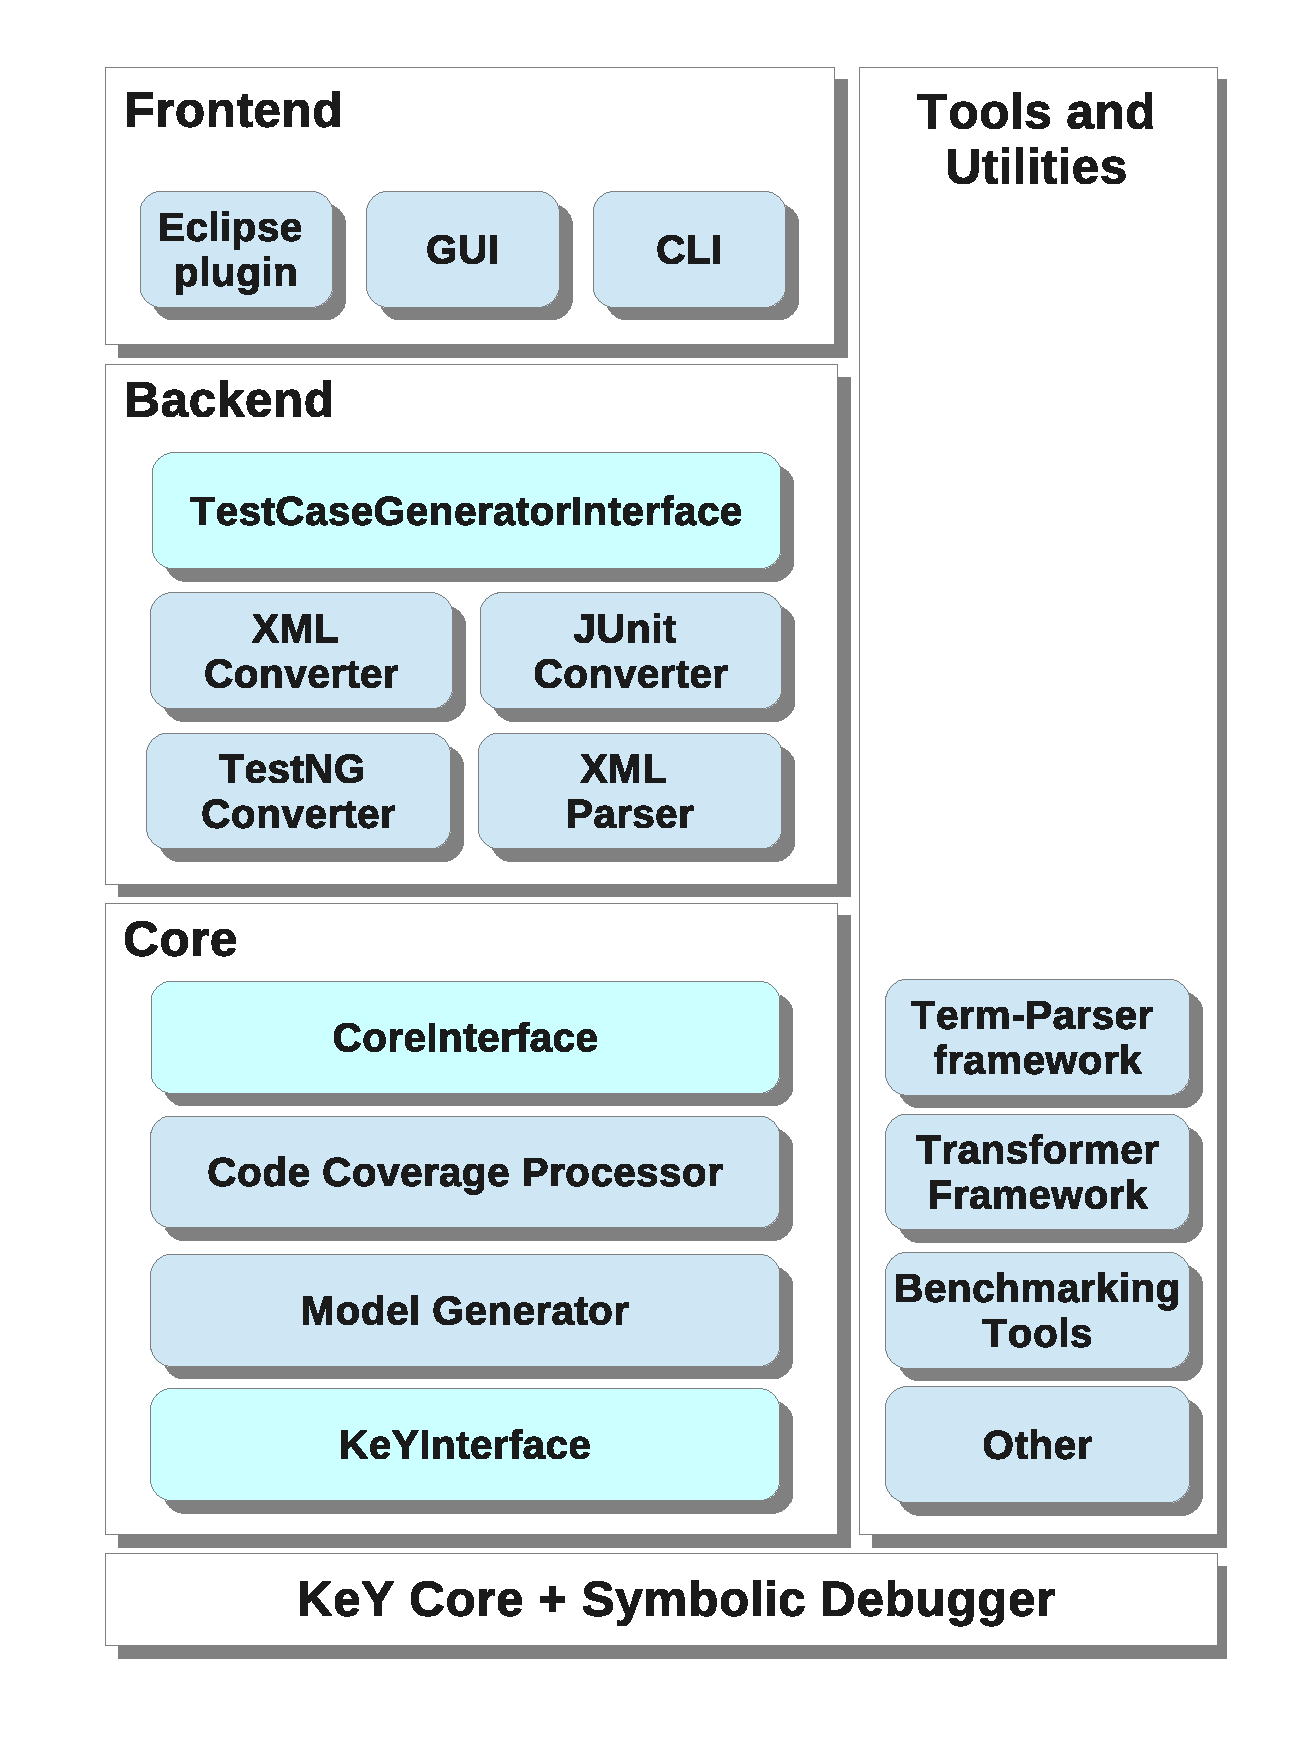
\includegraphics{KTG_Architecture.eps}}
        \caption{Architectural overview of KeYTestGen2}
      \end{figure}
    \end{tmparmod}
  \end{tmparmod}
\end{tmparmod}



\subsubsection{General architecture}

KeYTestGen2 is constructed following a layered, modular approach. Each
particular layer (Frontend, Backend, and Core) requests services from the
layer directly below it, and provides services for the layer above it (except
for the Frontend, which provides services directly to the user). The exception
to this rule is the Tools and Utilities module, which provides services
available to all the other layers.



Each of the primary layers provides a service interface for the layer above
it, providing a uniform API. Each such layer is implemented as a threadsafe
singleton.



To facilitate maintainability and extendability, The subsystems of each module
are largely interface based, making it easy to extend them with new
implementations. Further, the system has been implemented with concurrency in
mind, and each module should be able to operate in a multi-threaded
context{\footnote{Unfortunately, as will be discussed in the Evaluation, some
external dependencies to the system do not perform very well in this
setting.}}.



\subsubsection{Data flow}

The graph below illustrates, at a high level, the general pattern of dataflow
through KeYTestGen2. While the system is targeted to support several test
frameworks, we here use JUnit as an example.



\begin{figure}[h]
  \resizebox{15cm}{!}{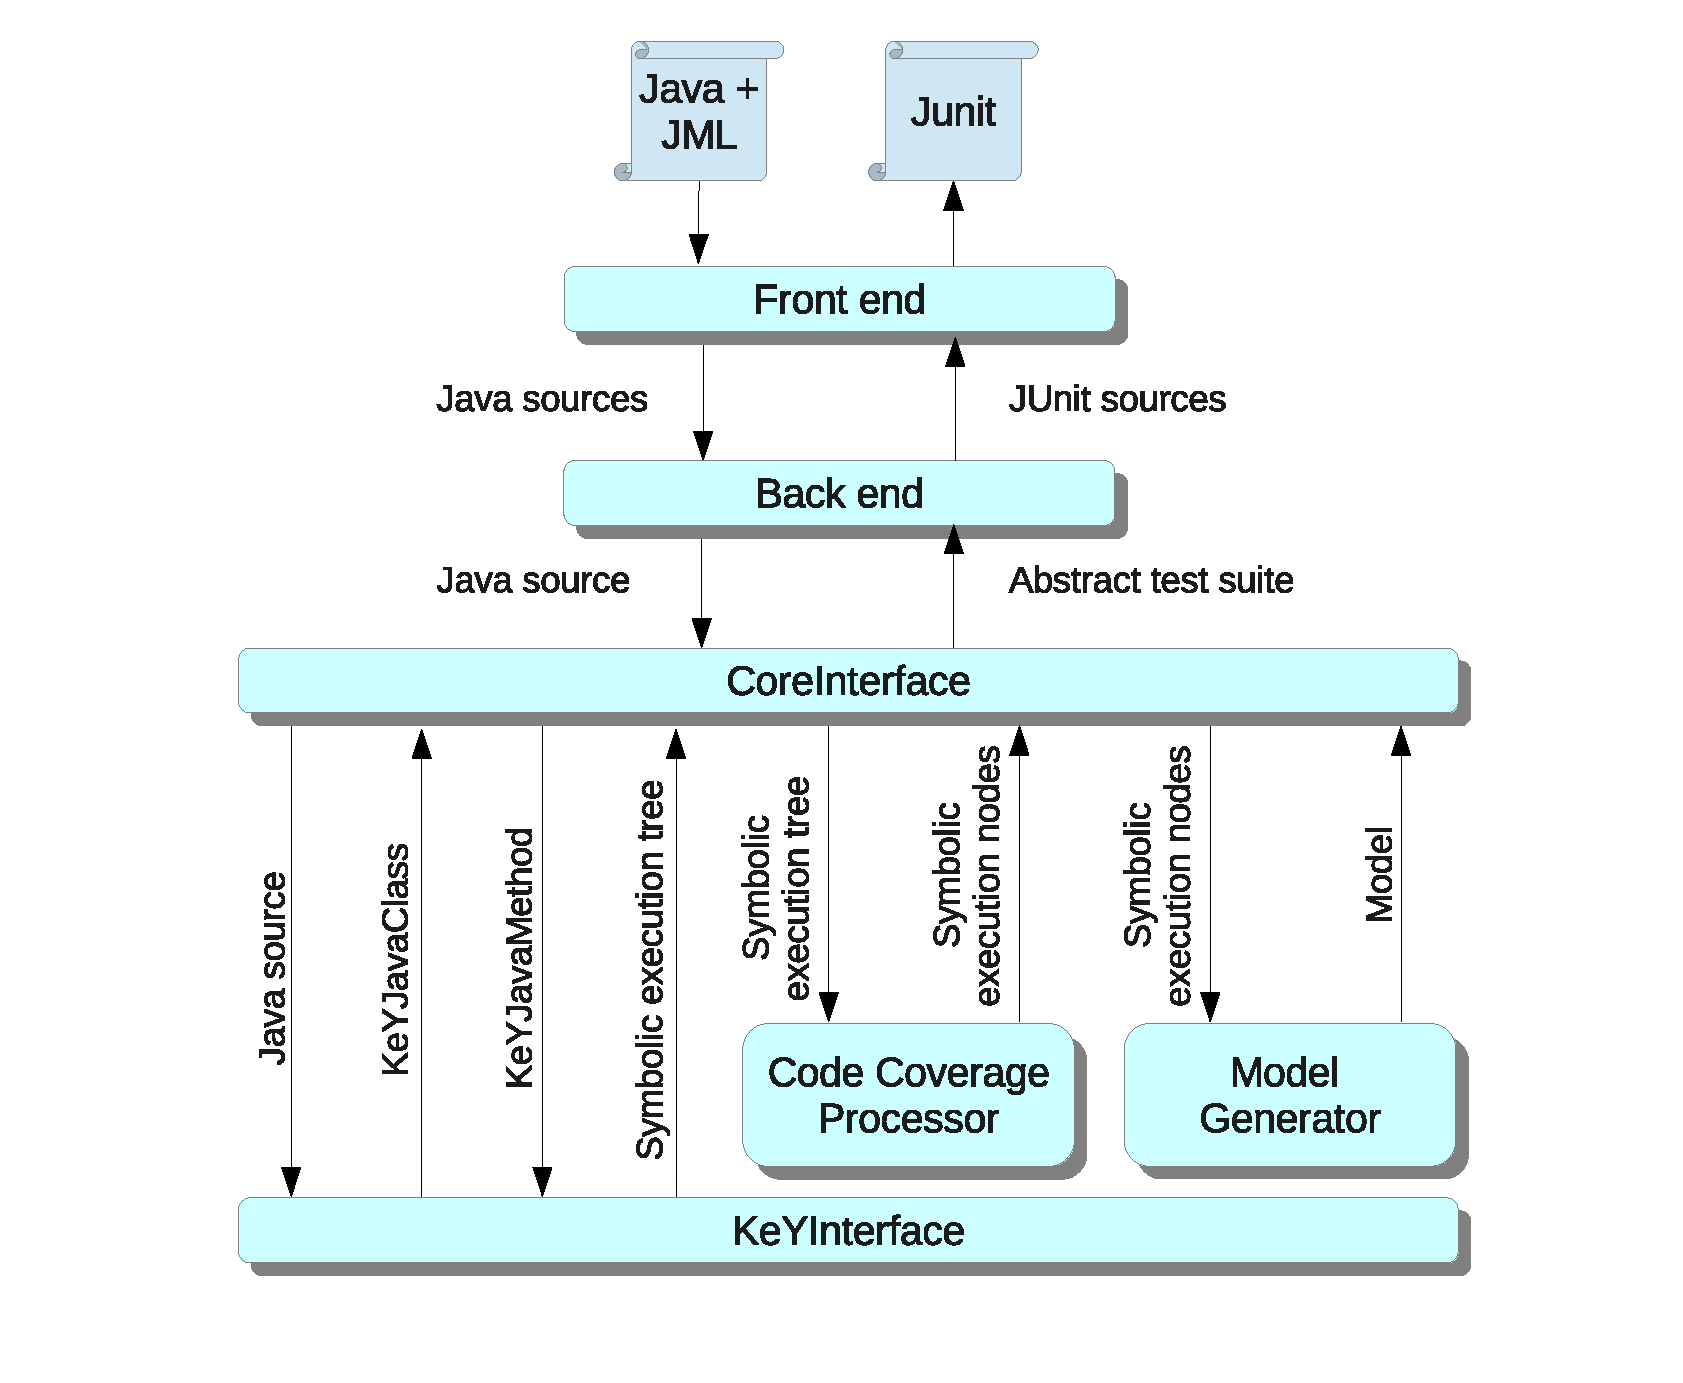
\includegraphics{KTG_Dataflow.eps}}
  \caption{Data flow model for KeYTestGen2.}
\end{figure}



\subsubsection{Core}

The core system provides central services related to test case generation,
including the creation of symbolic execution trees, generating models for the
same, and creating abstract test suites for encoding to specific frameworks.
Modules in this section are the following:
\begin{itemizedot}
  \item {\tmstrong{The KeY Interface}} - provides a central interface for
  KeYTestGen2 to interact with a runtime instance of KeY and its Symbolic
  Debugger. KeYTestGen2 uses this primarily to invoke the Symbolic Debugger in
  order to retrieve a symbolic execution trees for Java methods.
  
  \item {\tmstrong{The CoreInterface}} - provides a central interface between
  KeYTestGen2 and its various backend modules. Backend modules can use this
  interface in order to retrieve abstract test suites for Java methods.
  
  \item {\tmstrong{The Model Generator}} - consumes nodes in a symbolic
  execution tree, and generates models which satisfiy their path conditions.
  
  \item {\tmstrong{The Code Coverage Processor}} - consumes a symbolic
  execution tree, and extracts from it the symbolic execution nodes needed in
  order to reach a certain degree of code coverage. Each such node will
  provide the foundation for a single test case.
\end{itemizedot}


\subsubsection{Backend}

The backend consists of a set of output generators, which conssume the
abstract test suites produced by KeYTestGen2, and convert them to some final
format. As of current, the KeYTestGen2 backend has near-complete support for
JUnit and XML outputs, and targeted support for TestNG. Adding additional
generators is simple.



\subsubsection{Frontend}

KeYTestGen2 has projected support both for CLI and GUI usage. The CLI is based
on JCommander, whereas the GUI uses standard Java Swing.

\subsection{The Core}

The role of the core system is to consume Java source files, gather data about
them through symbolic execution, and finally create a set of abstract test
suites based on this information. These test suites cam in turn be passed to
the various backend implementations for encoding to specific test frameworks.



\begin{tmparmod}{2cm}{0pt}{0pt}
  \begin{tmparmod}{2cm}{0pt}{0pt}
    \begin{tmparmod}{0pt}{2cm}{0pt}
      
      
      \begin{figure}[h]
        \includegraphics{KeYTestGen2-2.eps}
        \caption{The Core of KeYTestGen2.
        
        }
      \end{figure}
    \end{tmparmod}
  \end{tmparmod}
\end{tmparmod}



This process is realized through the interplay of the three central subsystems
of the Core; the KeYInterface, Code Coverage Parser (CCP), and Model
Generator. Here, we will study the inner workings of these three subsystems,
within the larger context of the functionality of the Core as a whole.

\begin{center}
  
\end{center}

\begin{center}
  \begin{tmparmod}{1cm}{0pt}{0pt}
    \begin{tmparmod}{0pt}{2cm}{0pt}
      
    \end{tmparmod}
  \end{tmparmod}
\end{center}

\subsubsection{The KeYInterface}

The KeYInterface acts as a service bridge between KeYTestGen2 and the rest of
KeY, allowing processes and modules in KeYTestGen to request services from the
rest of the KeY system.



Importantly, the KeYInterface retrieves symbolic execution trees for Java
methods. To do so, it uses the Symbolic Debugger of KeY. The configuration of
the Debugger itself is handled dynamically by the interface for each
invocation, in an attempt to optimize performance and the quality of the
resulting symbolic execution tree. \



\subsubsection{The Model Generator}

The role of the Model Generator is to consume a single symbolic execution
node, and create a {\tmem{model}} satisfying the path condition of that node.
This model is encoded as an {\tmem{abstract heap state}} (AHS, see below), and
can subsequently be turned into a specific test fixture by the backend.



The Model Generator achieves this in two steps:
\begin{itemize}
  \item The path condition of the node is analyzed in order to map constraints
  on the program variables involved. These constraints are then encoded as an
  AHS containing all program variables.
  
  \item If the mapping of constraints in stage 1 revealed any constraints on
  primitive-type variables, these constraints are isolated, encoded to an SMT
  formula, and passed to an SMT solver{\footnote{The current implementation
  uses the Microsoft Z3 solver by default. However, support for other solvers
  exists by virtue of KeY itself supporting them. Experimental support for
  using interal solvers (i.e. solvers implemented in Java and executing under
  the control of KeY) exists as well.}} to be resolved. The output od the SMT
  solver is then parsed to extract the value assignments satisfying the
  constraint, and these values are finally inserted back into their respective
  variables in the AHS. \
  
  
\end{itemize}
An {\tmstrong{abstract heap state}} is a simple abstraction of a Java heap
during runtime. It consists of three principal classes:


\begin{itemizedot}
  \item {\tmstrong{Model}} - corresponds to the model - and hence the abstract
  heap state itself. A Model encapsulates a set of related ModelVariables and
  ModelInstances, \ and provides a set of utility methods for working with
  them. Instances of this class constitute the principal output of the Model
  Generator.
  
  \item {\tmstrong{ModelVariable}} - corresponds to a Java variable, and has
  the following fields:
  \begin{itemizeminus}
    \item {\tmstrong{identifier : String}}, corresponding to the source-level
    name of the variable.
    
    \item {\tmstrong{type : String}}, corresponding to the name of the
    variables declared type.
    
    \item {\tmstrong{value : Object}}, corresponding to the runtime value
    referred by the variable. The dynamic type of the value can differs
    depending on the type of the variable itself:
    \begin{itemizearrow}
      \item {\tmstrong{A wrapper type}}{\footnote{I.e. Boolean, Integer,
      Float, Double, Byte or Character.}}, iff. the ModelVariable symbolizes a
      variable of primitive type, such as an interger or boolean.
      
      \item {\tmstrong{A ModelInstance}} or {\tmstrong{null}}, iff. the
      ModelVariable symbolizes a reference type.
    \end{itemizearrow}
  \end{itemizeminus}
  \item {\tmstrong{ModelInstance}} - corresponds to a dynamically created Java
  object, and has the following defining fields:
  \begin{itemizeminus}
    \item {\tmstrong{identifier : String}}, corresponding, loosely, to the
    memory reference of the object during runtime. In practice, it serves
    simply as a unique identifier (as a physical memory address must be
    unique).
    
    \item {\tmstrong{type : String}}, corresponding to the name of the type of
    the object.
    
    \item {\tmstrong{fields : List<ModelVariable>}}, corresponding to a subset
    of the fields of the object. The only fields expressed here are those
    needed to express a heapstate which satisfies the path condition the model
    of this ModelInstance is associated with.
    
    
  \end{itemizeminus}
\end{itemizedot}
We illustrate the process of Model Generation by looking at how it is done for
an example Java method.



\begin{tmparmod}{1cm}{0pt}{0pt}
  \begin{tmparmod}{0pt}{1cm}{0pt}
    {\noindent}{\noindent}\begin{tabular}{l}
      \begin{example}
        A Java method dealing only with primitive values.
        
        {\noindent}\begin{tmindent}
          \begin{tmparsep}{0em}
            public class Mid \{
            
            \ \ \
            
            \ \ \ // Returns the middle value of three integers
            
            \ \ \ public int mid(int x, int y, int z) \{
            
            \ \ \ \ \ \ int mid = z;
            
            \ \ \ \ \ \ if(y < z) \{
            
            \ \ \ \ \ \ \ \ \ \ if(x < y) \{
            
            \ \ \ \ \ \ \ \ \ \ \ \ \ \ mid = y;
            
            \ \ \ \ \ \ \ \ \ \ \} else if(x < z) \{
            
            \ \ \ \ \ \ \ \ \ \ \ \ \ \ mid = x; // <-- target statement
            
            \ \ \ \ \ \ \ \ \ \ \}
            
            \ \ \ \ \ \ \} else \{
            
            \ \ \ \ \ \ \ \ \ \ if(x > y) \{
            
            \ \ \ \ \ \ \ \ \ \ \ \ \ \ mid = y;
            
            \ \ \ \ \ \ \ \ \ \ \} else if(x > z) \{
            
            \ \ \ \ \ \ \ \ \ \ \ \ \ \ mid = x;
            
            \ \ \ \ \ \ \ \ \ \ \}
            
            \ \ \ \ \ \ \}
            
            \ \ \ \ \ \ return mid; \ \ \ \ \ \ \ \ \ \ \ \ \
            
            \ \ \ \}
            
            \}
          \end{tmparsep}
        \end{tmindent}{\hspace*{\fill}}{\medskip}
      \end{example}
    \end{tabular}{\hspace*{\fill}}{\smallskip}
  \end{tmparmod}
\end{tmparmod}





Say we wish to generate a test case causing the first {\tmstrong{mid = x;}} in
the code to be executed. We may assume we already have the symbolic execution
node for this statement, and that its path condition is the following:

{\noindent}\begin{tmindent}
  \begin{tmparsep}{0em}
    \begin{alltt}
z >= 1 + y & y <= x & z >= 1 + x
\end{alltt}
  \end{tmparsep}
\end{tmindent}{\hspace*{\fill}}{\medskip}

The Model Generator will now process this path condition according to step one
above. After this is done, we end up with the following abstract heap state:



\begin{tmparmod}{3cm}{0pt}{0pt}
  \begin{tmparmod}{2cm}{0pt}{0pt}
    \begin{tmparmod}{0pt}{2cm}{0pt}
      \begin{figure}[h]
        \resizebox{10cm}{!}{\includegraphics{KeYTestGen2-3.eps}}
        \caption{A model, or abstract heap state for the node corresponding to
        the statement indicated in Example 10. This heap state is the result
        of the first step in the model generation process, and hence has no
        concrete values for any of the Integers yet.}
      \end{figure}
    \end{tmparmod}
  \end{tmparmod}
\end{tmparmod}





Recognizing that there are primitive-typed variables present in this
model{\footnote{Under the current implementation, this recognition comes as a
side-effect of the way the path condition is subsequently transformed for SMT
evaluation - a path condition containing no primitive constraints will simply
be simplified to {\tmstrong{null}}, in which case KeYTestGen2 does not proceed
with the second step.}}, KeYTestGen2 next proceeds to find concrete value
assignments for these variables. To do so, it first needs to
simplify{\footnote{The reason this simplification is done is to minimize the
complexity of the resulting SMT problem. Allowing non-primitive variables and
nested declarations proved to cause this complexity to explode exponentially,
and I was concerned that this might impact both the performance and
reliability of the model generator. As it is now, all needed information about
non-primitive types is already found in the abstract heap state, and hence
there is no reason to use the SMT solver for resolving anything except
primitive values, which it can do in a matter of milliseconds.}} the path
condition, as follows:


\begin{enumeratenumeric}
  \item  The path condition is transformed into a form which contains nothing
  but constraints on primitive variables.
  
  \item Further, KeYTestGen2 factors out the occurences of any nested
  variable declarations in the path condition, replacing them with single
  primitive variables with symbolic names (e.g. the nesting hierarchy
  MyClass.OtherClass.YetOtherClass.x, where x is an integer and MyClass etc
  are object instances, becomes a single integer variable named
  ``MyClass\_OtherClass\_YetOtherClass\_x'').
  
  \item Finally, the entire formula is negated. This is necessary since the
  value assignments will be produced by asking the SMT solver to provide a
  {\tmem{counter example}} to the formula we pass to it. Since a counter
  example to the negation of our formula will be an assignment that satisfies
  the formula itself, this will give us exactly what we are looking for.
\end{enumeratenumeric}


Having been simplified and processed, the path condition is finally translated
into an SMT formula, and passed to an external SMT solver. If succesful, the
SMT solver will return an assignment of values satisfying our
formula{\footnote{Since symbolic execution removes all unreachable execution
nodes, such a formula must always be satisfiable. Failure to find an
assignment is hence considered exceptional, and will cause KeYTestGen2 to
raise an exception and terminate.}}, which in our case could be the following:



\begin{center}
  {\tmstrong{x = 3
  
  y = 2
  
  z = 4}}
\end{center}





Inserting these into the model, we end up with the following, final model:



\begin{tmparmod}{2cm}{0pt}{0pt}
  \begin{tmparmod}{0pt}{2cm}{0pt}
    \begin{figure}[h]
      \resizebox{10cm}{!}{\includegraphics{KeYTestGen2-4.eps}}
      \caption{The previous model, with concrete integer values inserted.}
    \end{figure}
  \end{tmparmod}
\end{tmparmod}



Finally, this model is returned as the result of the Model Generator
invocation.



\subsubsection{The CoreInterface}

The CoreInterface provides an API for the Backend modules to request services
from the Core itself. It consumes the path to a Java source file, an instance
of ICodeCoverageParser to generate the desired level of code coverage (see
below), as well as the name of the method to generate a test suite for, and
returns an abstract test suite for the same method.



The abstract test suite mentioned above consists of the following classes:
\begin{itemizedot}
  \item {\tmstrong{TestSuite}} - the suite itself, as defined in section 2. It
  is a simple container class containing a reference to a KeYJavaMethod, as
  well as a set of TestCase instances.
  
  \item {\tmstrong{TestCase}} - represents a test case, as defined in section
  2. It consists of the following essential fields:
  \begin{itemizeminus}
    \item {\tmstrong{method : KeYJavaMethod}}, represents the method for which
    the test case is generated.
    
    \item {\tmstrong{model : Model}}, represents the model, or test fixture,
    for the test case.
    
    \item {\tmstrong{oracle : Term}}, represents the oracle of the test case.
    
    
  \end{itemizeminus}
\end{itemizedot}
Given the input values specificed in the beginning of this section, a test
suite is constructed in the following way:
\begin{enumeratenumeric}
  \item The KeYInterface and Core Utils are invoked in order to retrieve a
  KeYJavaClass instance for the target class.
  
  \item A symbolic execution tree for the target method is retrieved via the
  KeYInterface.
  
  \item The ICodeCoverageParser instance is applied to the symbolic execution
  tree in order to extract all nodes needed to generate a test suite
  fulfilling the level of code coverage tageted by the parser instance.
  
  \item A Thread pool is configured to concurrently generate models for the
  nodes. The results are pooled and, depending on configuration, the process
  terminates if any of the model generation threads fail.
  
  \item The results of the model generation are combined with the existing
  metada existing for the methods, and encoded into a set of TestCase
  instances.
  
  \item Finally, the TestCase instances generated in this fashion, along with
  existing data, are used to create a TestSuite instance.
\end{enumeratenumeric}


\subsubsection{The Code Coverage Parser (CCP)}

In order to provide code coverage for generated test cases, the symbolic
execution tree needs to be filtered in order to retrieve the nodes whose
execution will guarantee such coverage. This is the task of the CCP, which is
provided by the Core Utils.



Rather than being a single parser, the CCP provides a miniature framework for
implementing such parsers, consisting of the interface
{\tmstrong{ICodeCoverageParser}}. together with a set of utility classes for
working with IExecutionNode instances.

\subsection{The Backend}

The role of the backend is twofold. One the one hand, it consumes the abstract
test suites generated by the Core, converting them to some other format. On
the other hand, it also provides a uniform interface for the Frontend modules
to service the requests of users with regard to test case generation.



\begin{tmparmod}{2cm}{0pt}{0pt}
  \begin{tmparmod}{0pt}{2cm}{0pt}
    \begin{figure}[h]
      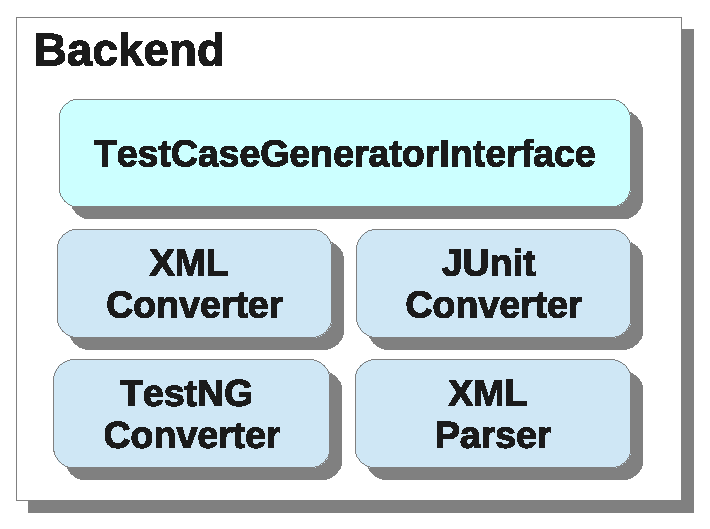
\includegraphics{Backend_Architecture.eps}
      \caption{The KeYTestGen2 Backend module, composed of the Test Suite
      Generator (towards the Frontend), default Converters, and tools for
      creating additional Converters (XML Parser).}
    \end{figure}
  \end{tmparmod}
\end{tmparmod}



\subsubsection{TestSuiteGenerator}

The interface seen by the Frontend is represented by the
{\tmstrong{TestSuiteGenerator}} singleton, which offers the following three
services to callers.
\begin{itemizedot}
  \item {\tmstrong{Generate test suites for a Java class}} - generates a set
  of test suites for the methods in a given Java class. Two implementations of
  this service are provided:
  \begin{itemizeminus}
    \item Generate a set of test suites covering only a specific
    {\tmstrong{subset}} of methods in the class, as specified by the user.
    
    \item Generate a set of test suites covering {\tmstrong{all}} methods in
    the class, giving the user the option to specify if such methods should
    include private methods, protected methods and/or methods inherited from
    java.lang.Object{\footnote{i.e. toString(), hashCode(), await(), notify(),
    notifyAll(), equals(Object other).}}
  \end{itemizeminus}
  \item {\tmstrong{Generate a test suite for a single symbolic execution
  node}} - this is provided not primarily for use by the Frontend, but as a
  hook for the Symbolic Debugger to use{\footnote{This functionality will be
  moved to a separate interface.}} (see section 5).
  
  
\end{itemizedot}
When invoking any of the services described above, the user can supply
implementations of the following interfaces, in order to control the outcome
of the test suite generation process:
\begin{itemizedot}
  \item {\tmstrong{IFrameworkConverter}} - to specify what framework/format
  the resulting test suites should be encoded to. If this is not specified,
  KeYTestGen2 will default to its native XML format.
  
  \item {\tmstrong{ICodeCoverageParser}} - to specify the level of code
  coverage to to achieve. If left unspecified, KeYTestGen2 will simply
  generate at least one test case for each return statement in the method. 
\end{itemizedot}


\subsubsection{Framework converters}

Support for output to specific test frameworks can be added by implementing
the IFrameworkConverter interface. These implementations can then simply be
passed to to the TestSuitGenerator as described in the previous section.



Currently, KeYTestGen2 aims to natively provide such implementations for
JUnit, TestNG, as well as a native XML format. This XML format is suitable for
users who wish to process the generated test suites in some other context than
KeYTestGen2 itself.



\subsubsection{Generating Java source files}

While it is technically deprecated{\footnote{Future iterations of KeYTestGen2
will use the template engine StringTemplate {\cite{StringTemplateWebsite}}}},
the Backend provides a utility class which can be overridden in order to write
formatted Java source code, called {\tmstrong{AbstractJavaSourceWriter}}. It
contains a relatively intuitive API, although the implementation is rather
clumsy and hence set apart for future replacement.



\subsection{The JUnit Converter}

As an example of how the previously discussed backend works, we will here
outline the JUnit Converter, responsible for converting abstract test suites
to JUnit ones.

\subsubsection{General structure}

The main stages in converting an abstract test suite to a JUnit one are the
following:
\begin{itemizedot}
  \item Create various utility methods within the JUnit test suite for use
  during testing.
  
  \item Create a test case for each test case represented in the abstract test
  suite:
  \begin{itemizeminus}
    \item Convert the Model of the test case to a JUnit fixture.
    
    \item Convert the Oracle of the test case to a set of JUnit assertions.
    
    \item Set up the execution of the method itself. \ 
  \end{itemizeminus}
\end{itemizedot}


Currently, the JUnit Converter uses KeYTestGen2s provided
AbstractJavaSourceWriter in order to turn the JUnit code generated in the
stages described above into an actual, executable test suite.



\subsubsection{Test fixture generation}

JUnit test fixtures are constructed through converting the Model structures
generated by KeYTestGen2 into corresponding Java declarations. This is done in
two stages:
\begin{itemizedot}
  \item Write the variable declaration,
  
  \item Write the variable instantiation, if any.
\end{itemizedot}
The first step is trivial, as it is simply a matter of inferring, from the
ModelVariable instance for the variable, the type, identifier and potential
modifiers for the variable. This is subsequently turned into a Java
declaration.



The second step is accomplished by recursively analyzing the Object instance
pointed to by the ModelVariable. If it is an instance of some wrapper type
(Integer, Boolean etc), it is written as-is, since its toString() method will
automatically yield a sufficient String representation of the value it
contains.

In the event that the value is a ModelInstance instead, the variable is
pointing to some reference type, which we will need to instantiate
accordingly. To do so, the Converter will analyze the general metadata for the
instance (type, identifier etc), as well as the fields it declares. These
fields will have to be instantiated as well, together with the current
instance, and inserted into it.



To do so, KeYTestGen2 sets up a {\tmem{fixture repository}}, which both
creates, configures and contains all necessary object instances needed by the
test cases in the test suite. The objects set up in this fashion are created
by a call to their no-args constructors{\footnote{The previous KeYTestGen used
additional tools, such as Objenesis {\cite{ObjenesisWebsite}} in order to
circumvent situations where objects do not provide a no-args constructor. This
is not fully implemented in KeYTestGen2 as of yet.}}. Subsequently, they are
configured by using Java Reflection to directly insert values into object
fields. Finally, KeYTestGen provides a generic method for retrieving objects
in the repository based on the type of the variable they are being assigned
to.



\subsubsection{Test oracle generation}

JUnit uses {\tmem{assertions}} in order to verify whether or not a JUnit test
case produces a desired post-state. These are simply methods which take some
kind of boolean expression{\footnote{Several different implementations are
provided for the sake of intuitive structuring of the test oracles. For
example, assertTrue(boolean exp) checks if exp evaluates to true, and
assertEquals(int expected, int givent) checks that two integer values are
indeed equal.}}, and fail the test case immediately if the expression
evaluates to false. Hence, in order to construct an oracle, the Converter
analyzes the Term corresponding to the postcondition for the method under
test, simplifies it, and then translates it into an equivalent set of
assertions.



The simplification mentioned above is done in order to produce as short and as
readable a set of assertions as possible. This is done by transforming the
Term in the following ways:
\begin{itemizedot}
  \item All operators, apart from the standard boolean and arithmetic ones,
  are removed from the Term, and replaced with an equivalent boolean
  expression using only the standard operators.
  
  \item The Term is put into {\tmstrong{Negation Normal Form}} - i.e. the only
  negations present in the Term are negations of literals. \ \
  
  \item The Term is put into {\tmstrong{Conjunctive Normal Form}} - this is
  done in order to get a Term which only consists of conjunctions of logical
  formulas. Each such conjunction can then be turned into a separate
  assertion, since they all must hold in order for the test case to pass.
  \begin{itemizeminus}
    \item A negative side effect of putting the Term into CNF is that it may
    make the Term more complex, by introducing additional sub-formulas to it.
    To work around this, KeYTestGen2 will search for and remove duplicate
    operands from all conjunctions and disjunctions in the Term.
  \end{itemizeminus}
  \item Finally, the Term is ``prettified'' by putting all occuring literals
  into a natural order wrt. the operator they are part of. For example, the
  conjunction {\tmem{b \&\& a \&\& d \&\& c}} is sort to become {\tmem{a \&\&
  b \&\& c \&\& d}}. The same manner of sorting is carried out for other
  operators.
\end{itemizedot}


After it has been simplified, the Term is turned into a String representation,
the conjunctions are extracted, and finally written as separate JUnit
assertions.



We refer to Appendix B for an example of a test suite generated in the way
described above.



\subsection{The Frontend}

The Frontend is the least constrained module of KeYTestGen2, and mostly just
encapsulates the various user interfaces{\footnote{It is also, as of the
writing of this, the least developed module.}}. Adding additional interfaces
is trivial, as the needed connectors are already present in the backend
module.



\begin{tmparmod}{2cm}{0pt}{0pt}
  \begin{tmparmod}{0pt}{2cm}{0pt}
    \begin{figure}[h]
      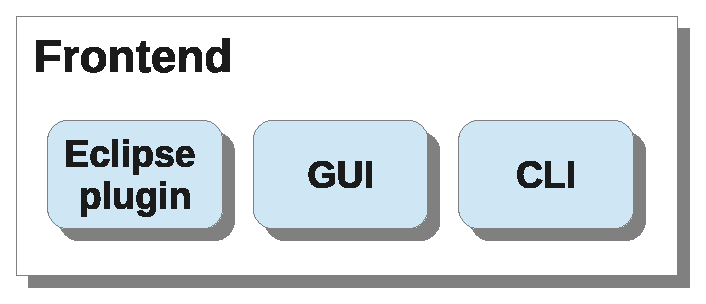
\includegraphics{Frontend_Architecture.eps}
      \caption{The KeYTestGen2 Frontend module, with the 3 default user
      interfaces.}
    \end{figure}
  \end{tmparmod}
\end{tmparmod}



\subsubsection{Provided user interfaces}

Natively, KeYTestGen2 provides the following user interfaces:
\begin{itemizedot}
  \item {\tmstrong{CLI}} - The command line interface is implemented using
  JCommander {\cite{JCommanderWebsite}}. It is aimed at being fully POSIX
  compliant, and support a wide array of features (see Appendix B).
  
  \item {\tmstrong{GUI}} - The graphical user interface will be implemented
  using the Java Swing framework. It will support the same basic functionality
  as the the CLI, while also offering the user visual feedback and the ability
  to execute third-party tools.
  
  \item {\tmstrong{Eclipse Plugin}} - Several KeY-based plugins for Eclipse
  exist already{\footnote{http://www.key-project.org/download/}}. While a
  separate one could be developed for KeYTestGen2{\footnote{This was actually
  done for the previous KeYTestGen, although it, like the project, is no
  longer maintained.}}, it is most likely more desirable that it is integrated
  with existing plugins. The Symbolic Debugger plugin in particular is already
  under serious consideration (see section 5).
\end{itemizedot}

\subsection{Tools and Utilities}

Tools and Utilities is a more loosely defined module than the others. It has
no central service interface, but rather contain a set of utilities which can
be used by all the other layers as needed.



\subsubsection{Term Tools}

Prominently, TaU contains a rich, lightweight tool kit for traversing and
transforming KeY Term instances. Such operations are formed extensively in the
processes of Model and Oracle Generation, for example.



Term transformers are easily implemented by overriding the abstract class
AbstractTermTransformer, and then simply overriding the methods modifying the
Terms one wishes to transform. For example, to modify Terms corresponding to
logical negations, one overrides the method {\tmstrong{transformNot(Term
term)}}.



While it is intuitive to use, this mini framework suffers from the immutable
nature of Terms - the modified nodes in a Term tree will have to be completely
replaced. As the kind of Terms KeYTestGen2 deals with are rather small, and
since object allocation in Java generally is not too expensive, this is not
such a serious drawback however.



\subsubsection{Benchmarking}

KeYTestGen2 features a rudimentary benchmarking tools, which allows following
and recording execution times for various parts of the system. This is useful
for testing, as well as debugging.

\section{Evaluation and future work}

Here, we provide reflections on the design and overall contribution of the
system, and give an overview of ongoing and future developments.

\subsection{Evaluation}

Here, we will briefly evaluate the current implementation of KeYTestGen2 with
regard to the four non-functional attributes described in section 4. We will
first evaluate the implementation in light of the non-functional attributes
outlined in section 5. Following that, we will summarize the current state of
the project as a whole.



\subsubsection{Fulfillment of non-functional requirements}

The driving non-functional attributes behind the evolution of KeYTestGen2, as
outlined in section 4, have so far been {\tmstrong{usability}},
{\tmstrong{maintainability}}, {\tmstrong{performance}}, and
{\tmstrong{reliability}}. Here, we will evaluate how KeYTestGen2 in its
current state meets them.
\begin{itemizedot}
  \item {\tmstrong{Usability}} - As the front end modules currently aren't
  fully implemented{\footnote{The CLI being partially implemented, the GUI and
  Eclipse plugin not at all.}}, the actual user interaction at this stage
  cannot be fully evaluated. What can be looked at, however, is the API and
  feature support.
  \begin{itemizeminus}
    \item One of the points of criticism by users of the previous KeYTestGen
    was the lack of options with regard to code coverage (KeYTestGen offering
    only MCDC). KeYTestGen2 addresses this by making it easy to specify
    different levels of coverage by implementing the ICodeCoverageParser
    interface in the Core.
    
    \item Another concern expressed by previous users was the lack of output
    options. KeYTestGen2 addresses this by making it easy to implement
    adapters for specific output formats, by providing basic interfaces and
    connectors for this task. Currently, KeYTestGen2 has native, preliminary
    support for JUnit and XML, with TestNG also being targeted for support.
    
    \item The API of the system Core is rather small at the moment (only 3
    public methods), but rich in functionality. The current services exported
    via the API allow for very customizable test generation sessions, where
    users can specify both code coverage, output format, as well as which
    methods of the target class to generate test cases for. Until more
    features are implemented, the API hardly needs to support more.
    
    \item KeYTestGen2 has been designed to be threadsafe, allowing it to be
    deployed in a multi-process environment. Bottlenecks do exist (primarily
    in the KeYInterface, which only allows one process at a time to access the
    KeY runtime), but these are likely to be addressed in future iterations.
    
    
  \end{itemizeminus}
  \item {\tmstrong{Maintainability}} - KeYTestGen2 has evolved with an
  increasing regard for separation of concerns between modules and individual
  subsystems. In terms of maintainability of the system, the following aspects
  are important:
  \begin{itemizeminus}
    \item Where applicable, most components define a clear data exchange
    format (such as the TestSuite abstraction for the Core, etc) for their
    output. This makes it easier to understand the dataflow within the system,
    as well as adding additional components consuming the same data.
    
    \item Many components (such as the Model Generator) are interface based,
    making it easy to plugin new implementations without extensive changes to
    the codebase.
    
    \item The code base is well documented, making it easy for newcomers and
    maintainers to understand, modify and extend it.
    
    \item The codebase is constantly being refactored and simplified,
    redundant solutions being factored out in favour of more concise and
    autonomous ones, making future modifications to it easier to decouple from
    their surrounding contexts.
    
    
  \end{itemizeminus}
  \item {\tmstrong{Performance}} - currently, this has proven to be the single
  most difficult attribute to address in KeYTestGen2. Even for trivial
  methods, execution times can easily run up to 30 seconds and
  beyond{\footnote{These numbers were obtained on a very powerful benchmark
  system (Intel i7 3939K, 16GB DDR3 RAM), which raise concenrs they might
  probably be much worse on more standard systems.}}, which borders on being
  unacceptable. Analysis of the of the KeYTestGen2 execution cycle has showed
  the following areas to be the largest bottlenecks:
  \begin{itemizeminus}
    \item {\tmstrong{Symbolic execution}} - due to the cost of running the KeY
    proof process, together with the overhead of subsequent symbolic execution
    tree construction, it is to be expected that this will take time.
    Furthermore, even {\tmem{loading}} the KeY system can take several seconds
    when running KeYTestGen2.
    
    \item {\tmstrong{Model Generation}} - the kind of SMT formulas generated
    by KeYTestGen2 are very simple{\footnote{Exclusively constraints on
    primitive types.}}, and should in general not take more than a few
    milliseconds for an SMT solver to complete. The real reason this part of
    the system runs slow appears to be related to overhead in executing the
    solvers themselves. KeYTestGen2 currently makes use of the standard KeY
    SMT interface, which involves creating a fair number of threads, as well
    setting up external OS processes in order to invoke a solver.
    
    
  \end{itemizeminus}
  Suggestions for how to address these can be found under ``future work''
  below. On the positive side of things, the following aspects of KeYTestGen2
  have a positive impact on performance:
  
  
  \begin{itemizeminus}
    \item The system is designed with simplicity in mind. While it makes heavy
    use of abstractions, it also aims to create as few objects as possible
    during runtime, minimizing overhead and memory usage.
    
    \item Wherever tasks can be performed in parallel, this is being taken
    advantage of. Model generation for several execution nodes, for example,
    is done in a completely concurrent manner.
  \end{itemizeminus}
  
  
  \item {\tmstrong{Reliability}} - apart from testing, there is so far no
  rigorous checking that the output of KeYTestGen2 corresponds to what is
  expected by the user. This will need to addressed. Being part of KeY, it is
  reasonable that this should be done through formal verification of
  KeYTestGen2 via KeY, at least for methods which could be considered
  critical.
\end{itemizedot}


\subsubsection{Overall assessment}

KeYTestGen is under continous development. The version presented as a part of
this thesis at best represents a primitve proof of concept for what the
project could (and, all things going well, will) potentially grow into.



That said, much of the essential aspects of the system are at least partially
implemented. It is possible, for example, to generate both JUnit and XML test
suites for many simple methods{\hspace{0.0em}}{\footnote{I.e. methods not
calling other methods, not containing any loop structures, and using only
primitive and/or user-defined object types with no-param constructors.}}.



\subsection{Could we create useful test suites?}

Before we go on to discuss other upcoming work, there is one particular issue
deserving of special attention. It is the question of whether or not we can
really generate {\tmem{useful}} test suites in an automatic fashion - an
important factor in estimating just how appropriate KeYTestGen2 might be for
an industrial context.



As can be seen in this work, while the current{\footnote{Here, we mean the
output of the resident test suite converters, in particular the JUnit one.}}
output of KeYTestGen satisfies many {\tmem{technical}} quality measures (such
as code coverage), it leaves very much to be desired in terms
{\tmem{non-technical}} qualities. An example of the latter would be
{\tmem{code readability}}, which we consider below



\subsubsection{Code readability}

One of the great benefits of unit testing is that test cases can serve as a
form of documentation for the system under test. Each test case demonstrates
the (correct) operation of a given aspect of the system as a whole (i.e. a
unit), and can thus be very helpful both for existing and new
developers{\footnote{Or customers, for that matter.}} to learn about how it
works. Ideally, just as for normal code, the code of test cases should richly
documented{\footnote{In terms of comments and JavaDoc.}} in order to make such
understanding even easier.



KeYTestGen2 is currently {\tmem{not}} able generate such test cases, and this
is rooted in the fact that it does not really ``understand'' the way states
are formed in the Java code it generates.



This is most visible in the way which KeYTestGen2 translates abstract heap
states to concrete ones. As we have shown in section 4, this process is
strictly mechanical, and KeYTestGen2 will make use of direct-access tools such
as reflection and Objenesis in order to {\tmem{directly}} create and
manipulate fields of objects on the heap. The problem here is that KeYTestGen2
completely {\tmem{misses}} the {\tmem{natural patterns}} involved in bringing
the system from one state to another. The best it can do is to create an
artificial state {\tmem{in situ}}.

The result of this process is code that a human being most likely would
{\tmem{never}} write, and hence, code which a human being most likely might
not find all too useful to read either.



To illustrate, consider the simple class below, representing a piece in some
board game:



\begin{tmparmod}{1cm}{0pt}{0pt}
  \begin{tmparmod}{0pt}{1cm}{0pt}
    {\noindent}{\noindent}\begin{tabular}{l}
      \begin{example}
        A simple game board piece.
        
        {\noindent}\begin{tmindent}
          \begin{tmparsep}{0em}
            public class BoardPiece \{
            
            \ \ \ // ...
            
            \ \ \ private int moves;
            
            \ \ \ private int xCord;
            
            \ \ \ private int yCord;
            
            
            
            \ \ \ public BoardPiece() \{
            
            \ \ \ \ \ \ \ xCord = yCord = moves = 0;
            
            \ \ \ \}
            
            
            
            \ \ \ public moveUp \{
            
            \ \ \ \ \ \ \ ++moves;
            
            \ \ \ \ \ \ \ ++yCord;
            
            \ \ \ \}
            
            
            
            \ \ \ public moveRight \{
            
            \ \ \ \ \ \ \ ++moves;
            
            \ \ \ \ \ \ \ ++xCord
            
            \ \ \ \}
            
            \ \ \ // ...
            
            \}
          \end{tmparsep}
        \end{tmindent}{\hspace*{\fill}}{\medskip}
      \end{example}
    \end{tabular}{\hspace*{\fill}}{\smallskip}
  \end{tmparmod}
\end{tmparmod}





Imagine that we want to set up a heap state where this piece has been moved,
say, twice right, twice up, and the twice right again. The ``natural'' way of
reaching this state is illustrated below, followed by the same state generated
by KeYTestGen2.



\begin{tmparmod}{1cm}{0pt}{0pt}
  \begin{tmparmod}{0pt}{1cm}{0pt}
    {\noindent}{\noindent}\begin{tabular}{l}
      \begin{example}
        A ``naturally'' created test fixture
        
        {\noindent}\begin{tmindent}
          \begin{tmparsep}{0em}
            @Test
            
            public void TestBoardPieceMove() \{
            
            \ \ \
            
            \ \ \ // ...
            
            \ \ \ BoardPiece piece = new BoardPiece();
            
            \ \ \
            
            \ \ \ piece.moveRight();
            
            \ \ \ piece.moveRight();
            
            \ \ \
            
            \ \ \ piece.moveUp();
            
            \ \ \ piece.moveUp();
            
            \ \ \
            
            \ \ \ piece.moveRight();
            
            \ \ \ piece.moveRight();
            
            \ \ \ // ...
            
            \}
          \end{tmparsep}
        \end{tmindent}{\hspace*{\fill}}{\medskip}
      \end{example}
    \end{tabular}{\hspace*{\fill}}{\smallskip}
  \end{tmparmod}
\end{tmparmod}





\begin{tmparmod}{1cm}{0pt}{0pt}
  \begin{tmparmod}{0pt}{1cm}{0pt}
    {\noindent}{\noindent}\begin{tabular}{l}
      \begin{example}
        The same fixture generated by KeYTestGen2.
        
        {\noindent}\begin{tmindent}
          \begin{tmparsep}{0em}
            @Test
            
            public void TestBoardPieceMove() \{
            
            \ \ \ // ...
            
            \ \ \
            
            \ \ \ BoardPiece piece = getObjectInstance(41);
            
            
            
            \ \ \ // ...
            
            \}
            
            
            
            // ...
            
            
            
            objectInstances.put(41, new BoardPiece());
            
            
            
            // ...
            
            
            
            \{
            
            \ \ \ Boardpiece instance = getObjectInstance(41); \ \ \ \ \
            
            \ \ \ setFieldValue(instance, "xCord", 4);
            
            \ \ \ setFieldValue(instance, "yCord", 2);
            
            \}
          \end{tmparsep}
        \end{tmindent}{\hspace*{\fill}}{\medskip}
      \end{example}
    \end{tabular}{\hspace*{\fill}}{\smallskip}
  \end{tmparmod}
\end{tmparmod}



\

That the ``natural'' code is more expressive hardly needs justification. It
gets worse, however. Notice that the fixture directly generated by KeYTestGen2
does {\tmem{not even set the}} {\tmstrong{{\tmem{}}moves}} {\tmem{field}},
while the natural code does so as a part of invoking the
{\tmstrong{moveLeft()}} and {\tmstrong{moveRight()}} methods. In other words,
we end up with two states which are {\tmem{not even equivlanent}}.



This need not be as bad as it seems at first - if KeYTestGen2 had
{\tmem{needed}} the {\tmstrong{moves}} field to be set, then it would have
discovered this while analysing the path condition during model generation.
However, this necessity is only based on the execution run specificed by the
path condition - and we are in either case still left with {\tmstrong{piece}}
in a state which at least informally violates its functional contract with
regard to its implementation.



To overcome these difficulties, we will need to make KeYTestGen ``understand''
how to put a program in a given state, using nothing but the methods the
program itself provides in order to do so. While we do not have a clear idea
for how this could be done, it will certainly involve deep introspection with
regard to the Java code of the system under test, and possibly aspects of
machine learning. The potential complexity of enabling this makes it a worthy
project on its own, separate from any other developments related to
KeYTestGen2 itself{\footnote{Yes, I am more or less certain what I will be
doing for my master thesis as this is being jotted down.}}.

\subsection{Future work}

Below, we outline some of the more interesting aspects of current and future
work on KeYTestGen2.



\subsubsection{Reducing external dependencies}

The current implementation of KeYTestGen2 depends on SMT solvers in order to
perform model generation. It is desirable to get rid of this dependency, since
it occurs an unreasonable overhead{\footnote{The model generation process is
currently the most time consuming aspect of the execution cycle of
KeYTestGen2, the largest bottleneck being launching, waiting for, and
gathering results from external solvers.}} (translation to SMT formulas,
launching of OS processes for external solvers, etc) for solving what are
relatively simple problems, consisting almost exclusively of integer
constraints.



The natural way to solve this would be to provide a native
solution{\footnote{One attempt to circumvent this problem was to extend KeY to
support {\tmem{embedded}} SMT solvers as part of KeY:s SMT interface. Together
with this, the SMTInterpol solver was embedded into KeY as a separate project
(KeYnterpol) in order to provide a basis for benchmarking. Sadly, this setup
turned out to function almost as poorly as its external counterparts in
concurrent runs, while being only slightly better in single-threaded
performance.}}. Several constraint programming solvers implemented in Java
already exist - two prominent ones being JaCoP and Choco. Investigations are
ongoing to see how these could be integrated into KeYTestGen2.



\subsubsection{Code coverage}

\begin{flushleft}
  In its current state, KeYTestGen2 only generates test suites providing a
  primitive kind of statement coverage. To make it useful in actual
  development, it is desireable to provide at the very least the common
  forms{\footnote{i.e. statement, branch, condition and decision coverage.}},
  as well as at least one industrial-grade coverage criteria, such as MC/DC. 
\end{flushleft}



To facilitate this, algorithms need to be developed which can isolate the
execution needed for satisfying such criteria. I are not aware of any such
algorithms at this stage (and if they exist, they are most likely language
specific). If they need to be developed from scratch, it seems we are
essentially faced with two possibilities:
\begin{itemizedot}
  \item we work {\tmem{directly}} with the symbolic execution tree as-is. The
  downside of this is that execution trees can be enormously large, and
  algorithms based on tree-traversal may perform very poorly in this context.
  
  \item We construct an intermediate abstraction, and operate on this one. For
  example, we could condense the symbolic execution tree into an ``actual''
  execution graph (i.e. a standard graph representation of the statements in
  the code, and the transitions between them). The good thing about this is
  that it would most likely make the task of writing an algorithm simpler,
  since the underlying datastructure will be much simpler. On the downside,
  this still does not save us from the potential performance penalty of having
  to traverse the symbolic execution tree itself. Regardless, such traversal
  may be simpler in this case (since it only involves transformation), and
  overall performance may as such be better. 
\end{itemizedot}


\subsubsection{Input partitioning coverage}

To qualify as a complete glass box test case generator, KeYTestGen2 will need
to have facilities for generating test cases based on possible input
partitionings for the unit under test. There are several, state-of-the-art
black box test case generators which do so already, notably JMLUnitNG.
Investigations will be done to see how these two test case generation systems
could be unified into forming a single, glass box system.

\subsubsection{Improved user feedback}

Since KeYTestGen2 performs an extensive analysis of the source code it
consumes (due to symbolic execution), we see the possibility of the tool
providing extensive feedback to the user about the quality of the code, in
addition to generating test cases for it.



For example, the tool could potentially detect more subtle runtime errors
which are otherwise caught neither by the compiler nor signaled by exceptions
at runtime. One such case would be statements which are unreachable due to
their path conditions being unsatisfiable. Example 10 demonstrates one such
case.



\begin{tmparmod}{1cm}{0pt}{0pt}
  \begin{tmparmod}{0pt}{1cm}{0pt}
    {\noindent}{\noindent}\begin{tabular}{l}
      \begin{example}
        
        
        
        
        An unreachable statement: {\tmstrong{return x;}}
        
        {\noindent}\begin{tmindent}
          \begin{tmparsep}{0em}
            int a = 5;
            
            int b = 4;
            
            if(a > b) \{
            
            \ \ if(b > a) \{
            
            \ \ \ \ \ return x;
            
            \ \ \}
            
            \}
          \end{tmparsep}
        \end{tmindent}{\hspace*{\fill}}{\medskip}
      \end{example}
    \end{tabular}{\hspace*{\fill}}{\smallskip}
  \end{tmparmod}
\end{tmparmod}

\ \



Since a > b and a < b are mutually exclusive expressions, the statement
return x; can never be executed under normal conditions. Such anomalies are
certainly results of a mistake in the development process, and thus something
the developer would want to get notified about.



\subsubsection{KeY integration}

Integration of KeYTestGen with the main KeY system has been an objective from
the beginning. In particular, close integration between the Symbolic Debugger
of KeY and KeYTestGen has been targeted. From the perspective of the debugger,
KeYTestGen could be invoked in order to generate individual test cases for
specific execution nodes. From the perspective of KeYTestGen, the debugger
could, for example, be invoked dynamically in order to assist the user in
resolving situations where certain degrees of code coverage cannot be
satisfied due to errors in the design of th code itself.



\subsubsection{Support for more frameworks and test granularities}

Currently, KeYTestGen has partial support for generating test suites for the
JUnit framework. In the long term, we aim to implement support for other test
frameworks as well, with TestNG {\cite{TestNGwebsite}} being the current
target.



It is noteworthy that both JUnit and TestNG are primarily designed for unit
testing. As far as possible, it would be interesting to explore the
possibilities of generating test cases of higher granularity, such as
integration tests. Doing so would of course require much more indepth analysis
of the code itself, along with possible manual input from the user (such as
specifications on class integration, etc).

\section{Conclusion}

Automated test case generation tools can provide a significant productivity
boost to modern software engineering processes, since they allow the otherwise
time consuming verification and validation phases to be automated. More
advanced such systems can confer even greater benefits, such as producing test
suites which guarantee certain levels of code coverage.



KeYTestGen2 is one such tool, being an extensible test case generation system
based on the symbolic execution technology of the KeY system. Using this
technology, KeYTestGen2 is capable of deriving a rich set of metadata about
possible execution paths through a software system. This data can then be
processed into a set of test suites, which may finally be encoded as test
suites for specific test frameworks such as JUnit or TestNG.



This work has described the the concepts behind KeYTestGen2, as well as the
precursor to it, KeYTestGen1. It has further explored the requirements and
implementation of the system, provided an evaluation of its current state, and
provided a summary of ongoing and future work on the system.



There is not yet a silver bullet for verification of software, but it is my
hope that KeYTestGen2 may eventually play a significant role in making that
process much more convenient. In the end, may it allow programmers to focus on
the one thing that has driven software development throughout the ages -
solving problems.



\section{Appendix A - KeYTestGen requirements.}

The following requirements have been adapted from an internal Chalmers
document{\footnote{Not cited or reproduced in its entirety for confidentiality
reasons. The project is not run by Chalmers.}} , outlining a formal set of
requirements on KeYTestGen with regard to a project Chalmers was participating
in at the time.



The requirements have been edited so as to exclude certain cases which were
relevant only for the project in question, but not general use.



These requirements are an interesting reference as they specify conditions
for KeYTestGen being applicable in an industrial context, which is also
something we target for KeYTestGen2. To the best of my knowledge, they are the
only extant formal requirements ever written for the system.

\subsection{Test Case Inputs}

This section analyses the problem of finding inputs for the test suite to
generate.



\subsubsection{User Requirements} \



{\tmstrong{Requirement 6.1: Generation of input values}}
\begin{enumeratealpha}
  \item The system {\tmstrong{shall}} generate test case inputs automatically.
  
\end{enumeratealpha}


{\tmstrong{Rationale:}} Test generation provides the user with test inputs for
a test suite

automatically. Certain coverage criteria are met by construction, see (10.3).



{\tmstrong{Requirement 6.2:}} {\tmem{Coverage criteria}}
\begin{enumeratealpha}
  \item The inputs of the generated test cases {\tmstrong{shall}} achieve a
  strong hybrid coverage.
  
  \item The inputs of the generated test cases {\tmstrong{shall}} achieve the
  strong Modified Condition/Decision Coverage (MC/CD) coverage criterion.
\end{enumeratealpha}


{\tmstrong{Rationale}}:
\begin{itemizedot}
  \item Hybrid coverage means that the tests are covering w.r.t. different
  definitions of test adequacy criteria. The ones we consider are
  program-based, specification-based, and error-based.
  \begin{itemizedot}
    \item In {\tmstrong{program-based}} criteria the code is analysed (here by
    symbolical execution. Rep- resenting the set of possible executions as a
    directed graph with one entry point and one exit point, any path from the
    entry node and the exit node is a representation of an execution (which
    can also be unfeasible). Coverage is then defined by means of the
    relationship between the test set (that is a set of paths) and the graph
    defined.
    
    \item In {\tmstrong{specification-based criteria}} tests are extracted
    from the (formal) specification which provides inputs and desired outputs
    by means of pre- and post-condition. The coverage is defined by means of
    identification of categories in the domain of the input parameters and
    their relationship with the test set.
    
    \item In {\tmstrong{error-based criteria}} an input-space analysis is
    required, and can be done either by inspecting the code or speculating on
    the specification; the result is the parti- tioning of the input space.
    That partitioning helps to test the program on the more error-prone
    inputs; e.g. corner cases in floats. Thus the input space is partitioned,
    and the coverage is defined on the way test inputs are taken from this
    partition. The aim is to guarantee strong criterion in the different
    paradigms at once.
  \end{itemizedot}
  \item MC/CD criterion is one of the strongest program-based testing
  criteria. It is mentioned in the DO-178B standard as the criterion which
  ensures that Level A (Catastrophic) software is tested adequately.
\end{itemizedot}


\subsubsection{Technical Requirements}



{\tmstrong{Requirement 6.3:}} {\tmem{Generate test cases in JUNIT}}
\begin{enumeratealpha}
  \item Test generation {\tmstrong{shall}} result in test cases following the
  JUNIT standard.
\end{enumeratealpha}


{\tmstrong{Rationale:}} \ The tests should be executed automatically, using a
well established

technology.

\subsection{Test Oracle}

This section analyses the problem of generating oracles (see section 2) based
on formally specified Java code.



\subsubsection{User Requirements}

{\tmstrong{Requirement}} {\tmstrong{6.5}}{\tmstrong{:}} {\tmem{Generation of
oracles from specifications}}
\begin{itemizedot}
  \item The system {\tmstrong{shall}} generate oracles from the postcondition
  of the provided method specifications.
\end{itemizedot}
\ \ {\tmstrong{Rationale:}} to fully automate test result evaluation. \



\subsubsection{Technical Requirements}

{\tmstrong{Requirement 6.6:}} {\tmem{JUnit test suite output}}
\begin{itemizedot}
  \item The system {\tmstrong{shall}} output a test suite for the
  Implementation Under Test (IUT).
\end{itemizedot}


{\tmstrong{Rationale:}} \ JUnit is a broadly used testing framework
(www.junit.org) for Java

development.

\section{Appendix B - Input and output examples}

Here, we illustrate the operation of KeYTestGen2 with examples of generated
JUnit test suites for select Java methods.

\begin{example}
  
  
  
  
  Given the Java method below, KeYTestGen2 will generate the test suite
  following it.
  
  
  
  {\noindent}\begin{tmindent}
    \begin{tmparsep}{0em}
      /*@ public normal\_behavior \ \
      
      \ @ ensures
      
      \ \ \ ({\textbackslash}result == x) ||
      
      \ \ \ ({\textbackslash}result == y) ||
      
      \ \ \ ({\textbackslash}result == z ); \
      
      \ @ ensures
      
      \ \ \ (({\textbackslash}result <= y) \&\& ({\textbackslash}result <= z
      )) ||
      
      \ \ \ (({\textbackslash}result <= y) \&\& ({\textbackslash}result <= x
      )) ||
      
      \ \ \ (({\textbackslash}result <= x) \&\& ({\textbackslash}result <= z
      )); \ \ \ \ \
      
      \ @ ensures
      
      \ \ \ (({\textbackslash}result >= y) \&\& ({\textbackslash}result >= z
      )) ||
      
      \ \ \ (({\textbackslash}result >= y) \&\& ({\textbackslash}result >= x
      )) ||
      
      \ \ \ (({\textbackslash}result >= x) \&\& ({\textbackslash}result >= z
      )); \ \ \ \ \
      
      \ @*/ensures
      
      \ \ \ (({\textbackslash}result >= y) \&\& ({\textbackslash}result >= z
      )) ||
      
      \ \ \ (({\textbackslash}result >= y) \&\& ({\textbackslash}result >= x
      )) ||
      
      \ \ \ (({\textbackslash}result >= x) \&\& ({\textbackslash}result >= z
      ));@*/
      
      public static int mid(int x, int y, int z) \{
      
      \ \ \ int mid = z;
      
      \ \ \ if (y < z) \{
      
      \ \ \ \ \ \ \ if (x < y) \{
      
      \ \ \ \ \ \ \ \ \ \ \ mid = y;
      
      \ \ \ \ \ \ \ \} else if (x < z) \{
      
      \ \ \ \ \ \ \ \ \ \ \ mid = x;
      
      \ \ \ \ \ \ \ \}
      
      \ \ \ \} else \{
      
      \ \ \ \ \ \ \ if (x > y) \{
      
      \ \ \ \ \ \ \ \ \ \ \ mid = y;
      
      \ \ \ \ \ \ \ \} else if (x > z) \{
      
      \ \ \ \ \ \ \ \ \ \ \ mid = x;
      
      \ \ \ \ \ \ \ \}
      
      \ \ \ \}
      
      \ \ \ return mid;
      
      \}
    \end{tmparsep}
  \end{tmindent}{\hspace*{\fill}}{\medskip}
\end{example}

\begin{example}
  JUnit test suite generated for the example above.
  
  {\noindent}\begin{tmindent}
    \begin{tmparsep}{0em}
      import org.junit.*;
      
      import java.lang.reflect.*;
      
      import java.util.*;
      
      import
      de.uka.ilkd.key.testgeneration.targetmodels.PrimitiveIntegerOperations;
      
      
      
      public \ class Test\_PrimitiveIntegerOperations\_mid \{
      
      \ \ \
      
      \ \ \ @Test
      
      \ \ \ public void testmid0 () \{
      
      \ \ \ \ \ \ \ PrimitiveIntegerOperations self = getObjectInstance(2);
      
      \ \ \ \ \ \ \ int x = -1;
      
      \ \ \ \ \ \ \ int y = 0;
      
      \ \ \ \ \ \ \ int z = 1;
      
      \ \ \ \ \ \ \ int result = self.mid(x,y,z);
      
      \ \ \ \ \ \ \ Assert.assertTrue(
      
      \ \ \ \ \ \ \ \ \ \ \ (result == x) ||
      
      \ \ \ \ \ \ \ \ \ \ \ (result == y) ||
      
      \ \ \ \ \ \ \ \ \ \ \ (result == z)
      
      \ \ \ \ \ \ \ );
      
      \ \ \ \ \ \ \ Assert.assertTrue(
      
      \ \ \ \ \ \ \ \ \ \ \ (result >= x) ||
      
      \ \ \ \ \ \ \ \ \ \ \ (result >= y)
      
      \ \ \ \ \ \ \ );
      
      \ \ \ \ \ \ \ Assert.assertTrue(
      
      \ \ \ \ \ \ \ \ \ \ \ (result >= x) ||
      
      \ \ \ \ \ \ \ \ \ \ \ (result >= z)
      
      \ \ \ \ \ \ \ );
      
      \ \ \ \ \ \ \ Assert.assertTrue(
      
      \ \ \ \ \ \ \ \ \ \ \ (result >= x) ||
      
      \ \ \ \ \ \ \ \ \ \ \ (result >= y) ||
      
      \ \ \ \ \ \ \ \ \ \ \ (result >= z)
      
      \ \ \ \ \ \ \ );
      
      \ \ \ \ \ \ \ Assert.assertTrue(
      
      \ \ \ \ \ \ \ \ \ \ \ (result >= y) ||
      
      \ \ \ \ \ \ \ \ \ \ \ (result >= z)
      
      \ \ \ \ \ \ \ );
      
      \ \ \ \ \ \ \ Assert.assertTrue(
      
      \ \ \ \ \ \ \ \ \ \ \ (result <= x) ||
      
      \ \ \ \ \ \ \ \ \ \ \ (result <= y)
      
      \ \ \ \ \ \ \ );
      
      \ \ \ \ \ \ \ Assert.assertTrue(
      
      \ \ \ \ \ \ \ \ \ \ \ (result <= x) ||
      
      \ \ \ \ \ \ \ \ \ \ \ (result <= z)
      
      \ \ \ \ \ \ \ );
      
      \ \ \ \ \ \ \ Assert.assertTrue(
      
      \ \ \ \ \ \ \ \ \ \ \ (result <= x) ||
      
      \ \ \ \ \ \ \ \ \ \ \ (result <= y) ||
      
      \ \ \ \ \ \ \ \ \ \ \ (result <= z)
      
      \ \ \ \ \ \ \ );
      
      \ \ \ \ \ \ \ Assert.assertTrue(
      
      \ \ \ \ \ \ \ \ \ \ \ (result <= y) ||
      
      \ \ \ \ \ \ \ \ \ \ \ (result <= z)
      
      \ \ \ \ \ \ \ );
      
      \ \ \ \}
      
      \ \ \
      
      \ \ \ @Test
      
      \ \ \ public void testmid1 () \{
      
      \ \ \ \ \ \ \ PrimitiveIntegerOperations self = getObjectInstance(6);
      
      \ \ \ \ \ \ \ int x = -1;
      
      \ \ \ \ \ \ \ int y = -1;
      
      \ \ \ \ \ \ \ int z = 0;
      
      \ \ \ \ \ \ \ int result = self.mid(x,y,z);
      
      \ \ \ \ \ \ \ Assert.assertTrue(
      
      \ \ \ \ \ \ \ \ \ \ \ (result == x) ||
      
      \ \ \ \ \ \ \ \ \ \ \ (result == y) ||
      
      \ \ \ \ \ \ \ \ \ \ \ (result == z)
      
      \ \ \ \ \ \ \ );
      
      \ \ \ \ \ \ \ Assert.assertTrue(
      
      \ \ \ \ \ \ \ \ \ \ \ (result >= x) ||
      
      \ \ \ \ \ \ \ \ \ \ \ (result >= y)
      
      \ \ \ \ \ \ \ );
      
      \ \ \ \ \ \ \ Assert.assertTrue(
      
      \ \ \ \ \ \ \ \ \ \ \ (result >= x) ||
      
      \ \ \ \ \ \ \ \ \ \ \ (result >= z)
      
      \ \ \ \ \ \ \ );
      
      \ \ \ \ \ \ \ Assert.assertTrue(
      
      \ \ \ \ \ \ \ \ \ \ \ (result >= x) ||
      
      \ \ \ \ \ \ \ \ \ \ \ (result >= y) ||
      
      \ \ \ \ \ \ \ \ \ \ \ (result >= z)
      
      \ \ \ \ \ \ \ );
      
      \ \ \ \ \ \ \ Assert.assertTrue(
      
      \ \ \ \ \ \ \ \ \ \ \ (result >= y) ||
      
      \ \ \ \ \ \ \ \ \ \ \ (result >= z)
      
      \ \ \ \ \ \ \ );
      
      \ \ \ \ \ \ \ Assert.assertTrue(
      
      \ \ \ \ \ \ \ \ \ \ \ (result <= x) ||
      
      \ \ \ \ \ \ \ \ \ \ \ (result <= y)
      
      \ \ \ \ \ \ \ );
      
      \ \ \ \ \ \ \ Assert.assertTrue(
      
      \ \ \ \ \ \ \ \ \ \ \ (result <= x) ||
      
      \ \ \ \ \ \ \ \ \ \ \ (result <= z)
      
      \ \ \ \ \ \ \ );
      
      \ \ \ \ \ \ \ Assert.assertTrue(
      
      \ \ \ \ \ \ \ \ \ \ \ (result <= x) ||
      
      \ \ \ \ \ \ \ \ \ \ \ (result <= y) ||
      
      \ \ \ \ \ \ \ \ \ \ \ (result <= z)
      
      \ \ \ \ \ \ \ );
      
      \ \ \ \ \ \ \ Assert.assertTrue(
      
      \ \ \ \ \ \ \ \ \ \ \ (result <= y) ||
      
      \ \ \ \ \ \ \ \ \ \ \ (result <= z)
      
      \ \ \ \ \ \ \ ); \ \ \
      
      \ \ \ \}
      
      \ \ \
      
      \ \ \ @Test
      
      \ \ \ public void testmid2 () \{
      
      \ \ \ \ \ \ \ PrimitiveIntegerOperations self = getObjectInstance(4);
      
      \ \ \ \ \ \ \ int x = 0;
      
      \ \ \ \ \ \ \ int y = -1;
      
      \ \ \ \ \ \ \ int z = 0;
      
      \ \ \ \ \ \ \ int result = self.mid(x,y,z);
      
      \ \ \ \ \ \ \ Assert.assertTrue(
      
      \ \ \ \ \ \ \ \ \ \ \ (result == x) ||
      
      \ \ \ \ \ \ \ \ \ \ \ (result == y) ||
      
      \ \ \ \ \ \ \ \ \ \ \ (result == z)
      
      \ \ \ \ \ \ \ );
      
      \ \ \ \ \ \ \ Assert.assertTrue(
      
      \ \ \ \ \ \ \ \ \ \ \ (result >= x) ||
      
      \ \ \ \ \ \ \ \ \ \ \ (result >= y)
      
      \ \ \ \ \ \ \ );
      
      \ \ \ \ \ \ \ Assert.assertTrue(
      
      \ \ \ \ \ \ \ \ \ \ \ (result >= x) ||
      
      \ \ \ \ \ \ \ \ \ \ \ (result >= z)
      
      \ \ \ \ \ \ \ );
      
      \ \ \ \ \ \ \ Assert.assertTrue(
      
      \ \ \ \ \ \ \ \ \ \ \ (result >= x) ||
      
      \ \ \ \ \ \ \ \ \ \ \ (result >= y) ||
      
      \ \ \ \ \ \ \ \ \ \ \ (result >= z)
      
      \ \ \ \ \ \ \ );
      
      \ \ \ \ \ \ \ Assert.assertTrue(
      
      \ \ \ \ \ \ \ \ \ \ \ (result >= y) ||
      
      \ \ \ \ \ \ \ \ \ \ \ (result >= z)
      
      \ \ \ \ \ \ \ );
      
      \ \ \ \ \ \ \ Assert.assertTrue(
      
      \ \ \ \ \ \ \ \ \ \ \ (result <= x) ||
      
      \ \ \ \ \ \ \ \ \ \ \ (result <= y)
      
      \ \ \ \ \ \ \ );
      
      \ \ \ \ \ \ \ Assert.assertTrue(
      
      \ \ \ \ \ \ \ \ \ \ \ (result <= x) ||
      
      \ \ \ \ \ \ \ \ \ \ \ (result <= z)
      
      \ \ \ \ \ \ \ );
      
      \ \ \ \ \ \ \ Assert.assertTrue(
      
      \ \ \ \ \ \ \ \ \ \ \ (result <= x) ||
      
      \ \ \ \ \ \ \ \ \ \ \ (result <= y) ||
      
      \ \ \ \ \ \ \ \ \ \ \ (result <= z)
      
      \ \ \ \ \ \ \ );
      
      \ \ \ \ \ \ \ Assert.assertTrue(
      
      \ \ \ \ \ \ \ \ \ \ \ (result <= y) ||
      
      \ \ \ \ \ \ \ \ \ \ \ (result <= z)
      
      \ \ \ \ \ \ \ );
      
      \ \ \ \}
      
      \ \ \
      
      \ \ \ @Test
      
      \ \ \ public void testmid3 () \{
      
      \ \ \ \ \ \ \ PrimitiveIntegerOperations self = getObjectInstance(1);
      
      \ \ \ \ \ \ \ int x = 1;
      
      \ \ \ \ \ \ \ int y = 0;
      
      \ \ \ \ \ \ \ int z = 0;
      
      \ \ \ \ \ \ \ int result = self.mid(x,y,z);
      
      \ \ \ \ \ \ \ Assert.assertTrue(
      
      \ \ \ \ \ \ \ \ \ \ \ (result == x) ||
      
      \ \ \ \ \ \ \ \ \ \ \ (result == y) ||
      
      \ \ \ \ \ \ \ \ \ \ \ (result == z)
      
      \ \ \ \ \ \ \ );
      
      \ \ \ \ \ \ \ Assert.assertTrue(
      
      \ \ \ \ \ \ \ \ \ \ \ (result >= x) ||
      
      \ \ \ \ \ \ \ \ \ \ \ (result >= y)
      
      \ \ \ \ \ \ \ );
      
      \ \ \ \ \ \ \ Assert.assertTrue(
      
      \ \ \ \ \ \ \ \ \ \ \ (result >= x) ||
      
      \ \ \ \ \ \ \ \ \ \ \ (result >= z)
      
      \ \ \ \ \ \ \ );
      
      \ \ \ \ \ \ \ Assert.assertTrue(
      
      \ \ \ \ \ \ \ \ \ \ \ (result >= x) ||
      
      \ \ \ \ \ \ \ \ \ \ \ (result >= y) ||
      
      \ \ \ \ \ \ \ \ \ \ \ (result >= z)
      
      \ \ \ \ \ \ \ );
      
      \ \ \ \ \ \ \ Assert.assertTrue(
      
      \ \ \ \ \ \ \ \ \ \ \ (result >= y) ||
      
      \ \ \ \ \ \ \ \ \ \ \ (result >= z)
      
      \ \ \ \ \ \ \ );
      
      \ \ \ \ \ \ \ Assert.assertTrue(
      
      \ \ \ \ \ \ \ \ \ \ \ (result <= x) ||
      
      \ \ \ \ \ \ \ \ \ \ \ (result <= y)
      
      \ \ \ \ \ \ \ );
      
      \ \ \ \ \ \ \ Assert.assertTrue(
      
      \ \ \ \ \ \ \ \ \ \ \ (result <= x) ||
      
      \ \ \ \ \ \ \ \ \ \ \ (result <= z)
      
      \ \ \ \ \ \ \ );
      
      \ \ \ \ \ \ \ Assert.assertTrue(
      
      \ \ \ \ \ \ \ \ \ \ \ (result <= x) ||
      
      \ \ \ \ \ \ \ \ \ \ \ (result <= y) ||
      
      \ \ \ \ \ \ \ \ \ \ \ (result <= z)
      
      \ \ \ \ \ \ \ );
      
      \ \ \ \ \ \ \ Assert.assertTrue(
      
      \ \ \ \ \ \ \ \ \ \ \ (result <= y) ||
      
      \ \ \ \ \ \ \ \ \ \ \ (result <= z)
      
      \ \ \ \ \ \ \ );
      
      \ \ \ \}
      
      \ \ \
      
      \ \ \ @Test
      
      \ \ \ public void testmid4 () \{
      
      \ \ \ \ \ \ \ PrimitiveIntegerOperations self = getObjectInstance(3);
      
      \ \ \ \ \ \ \ int x = 1;
      
      \ \ \ \ \ \ \ int y = 1;
      
      \ \ \ \ \ \ \ int z = 0;
      
      \ \ \ \ \ \ \ int result = self.mid(x,y,z);
      
      \ \ \ \ \ \ \ Assert.assertTrue(
      
      \ \ \ \ \ \ \ \ \ \ \ (result == x) ||
      
      \ \ \ \ \ \ \ \ \ \ \ (result == y) ||
      
      \ \ \ \ \ \ \ \ \ \ \ (result == z)
      
      \ \ \ \ \ \ \ );
      
      \ \ \ \ \ \ \ Assert.assertTrue(
      
      \ \ \ \ \ \ \ \ \ \ \ (result >= x) ||
      
      \ \ \ \ \ \ \ \ \ \ \ (result >= y)
      
      \ \ \ \ \ \ \ );
      
      \ \ \ \ \ \ \ Assert.assertTrue(
      
      \ \ \ \ \ \ \ \ \ \ \ (result >= x) ||
      
      \ \ \ \ \ \ \ \ \ \ \ (result >= z)
      
      \ \ \ \ \ \ \ );
      
      \ \ \ \ \ \ \ Assert.assertTrue(
      
      \ \ \ \ \ \ \ \ \ \ \ (result >= x) ||
      
      \ \ \ \ \ \ \ \ \ \ \ (result >= y) ||
      
      \ \ \ \ \ \ \ \ \ \ \ (result >= z)
      
      \ \ \ \ \ \ \ );
      
      \ \ \ \ \ \ \ Assert.assertTrue(
      
      \ \ \ \ \ \ \ \ \ \ \ (result >= y) ||
      
      \ \ \ \ \ \ \ \ \ \ \ (result >= z)
      
      \ \ \ \ \ \ \ );
      
      \ \ \ \ \ \ \ Assert.assertTrue(
      
      \ \ \ \ \ \ \ \ \ \ \ (result <= x) ||
      
      \ \ \ \ \ \ \ \ \ \ \ (result <= y)
      
      \ \ \ \ \ \ \ );
      
      \ \ \ \ \ \ \ Assert.assertTrue(
      
      \ \ \ \ \ \ \ \ \ \ \ (result <= x) ||
      
      \ \ \ \ \ \ \ \ \ \ \ (result <= z)
      
      \ \ \ \ \ \ \ );
      
      \ \ \ \ \ \ \ Assert.assertTrue(
      
      \ \ \ \ \ \ \ \ \ \ \ (result <= x) ||
      
      \ \ \ \ \ \ \ \ \ \ \ (result <= y) ||
      
      \ \ \ \ \ \ \ \ \ \ \ (result <= z)
      
      \ \ \ \ \ \ \ );
      
      \ \ \ \ \ \ \ Assert.assertTrue(
      
      \ \ \ \ \ \ \ \ \ \ \ (result <= y) ||
      
      \ \ \ \ \ \ \ \ \ \ \ (result <= z)
      
      \ \ \ \ \ \ \ );
      
      \ \ \ \}
      
      \ \ \
      
      \ \ \ @Test
      
      \ \ \ public void testmid5 () \{
      
      \ \ \ \ \ \ \ PrimitiveIntegerOperations self = getObjectInstance(5);
      
      \ \ \ \ \ \ \ int x = 0;
      
      \ \ \ \ \ \ \ int y = 0;
      
      \ \ \ \ \ \ \ int z = 0;
      
      \ \ \ \ \ \ \ int result = self.mid(x,y,z);
      
      \ \ \ \ \ \ \ Assert.assertTrue(
      
      \ \ \ \ \ \ \ \ \ \ \ (result == x) ||
      
      \ \ \ \ \ \ \ \ \ \ \ (result == y) ||
      
      \ \ \ \ \ \ \ \ \ \ \ (result == z)
      
      \ \ \ \ \ \ \ );
      
      \ \ \ \ \ \ \ Assert.assertTrue(
      
      \ \ \ \ \ \ \ \ \ \ \ (result >= x) ||
      
      \ \ \ \ \ \ \ \ \ \ \ (result >= y)
      
      \ \ \ \ \ \ \ );
      
      \ \ \ \ \ \ \ Assert.assertTrue(
      
      \ \ \ \ \ \ \ \ \ \ \ (result >= x) ||
      
      \ \ \ \ \ \ \ \ \ \ \ (result >= z)
      
      \ \ \ \ \ \ \ );
      
      \ \ \ \ \ \ \ Assert.assertTrue(
      
      \ \ \ \ \ \ \ \ \ \ \ (result >= x) ||
      
      \ \ \ \ \ \ \ \ \ \ \ (result >= y) ||
      
      \ \ \ \ \ \ \ \ \ \ \ (result >= z)
      
      \ \ \ \ \ \ \ );
      
      \ \ \ \ \ \ \ Assert.assertTrue(
      
      \ \ \ \ \ \ \ \ \ \ \ (result >= y) ||
      
      \ \ \ \ \ \ \ \ \ \ \ (result >= z)
      
      \ \ \ \ \ \ \ );
      
      \ \ \ \ \ \ \ Assert.assertTrue(
      
      \ \ \ \ \ \ \ \ \ \ \ (result <= x) ||
      
      \ \ \ \ \ \ \ \ \ \ \ (result <= y)
      
      \ \ \ \ \ \ \ );
      
      \ \ \ \ \ \ \ Assert.assertTrue(
      
      \ \ \ \ \ \ \ \ \ \ \ (result <= x) ||
      
      \ \ \ \ \ \ \ \ \ \ \ (result <= z)
      
      \ \ \ \ \ \ \ );
      
      \ \ \ \ \ \ \ Assert.assertTrue(
      
      \ \ \ \ \ \ \ \ \ \ \ (result <= x) ||
      
      \ \ \ \ \ \ \ \ \ \ \ (result <= y) ||
      
      \ \ \ \ \ \ \ \ \ \ \ (result <= z)
      
      \ \ \ \ \ \ \ );
      
      \ \ \ \ \ \ \ Assert.assertTrue(
      
      \ \ \ \ \ \ \ \ \ \ \ (result <= y) ||
      
      \ \ \ \ \ \ \ \ \ \ \ (result <= z)
      
      \ \ \ \ \ \ \ );
      
      \ \ \ \}
      
      \ \ \
      
      \ \ \ private static HashMap<Integer, Object> objectInstances =
      
      \ \ \ \ \ \ \ new HashMap<Integer,Object>();
      
      
      
      \ \ \ /**
      
      \ \ \ \ * This method will retrieve an object instance corresponding \
      \ \ \ \
      
      \ \ \ \ * to its reference ID.
      
      \ \ \ \ */
      
      \ \ \ private static <T> T getObjectInstance (int reference) \{
      
      \ \ \ \ \ \ \ return (T)objectInstances.get(reference);
      
      \ \ \ \}
      
      \ \ \
      
      \ \ \ /**
      
      \ \ \ \ * Sets a field of some object to a given value
      
      \ \ \ \ */
      
      \ \ \ private static void setFieldValue (Object instance,
      
      \ \ \ \ \ \ \ String fieldName, Object value)
      
      \ \ \ \ \ \ \ throws NoSuchFieldException, SecurityException, \ \ \ \ \
      \ \ \ \ \ \ \ \ \ \ \ \ \ \ \ \ \
      
      \ \ \ \ \ \ \ \ \ \ \ IllegalArgumentException, IllegalAccessException
      \{
      
      \ \ \ \ \ \ \
      
      \ \ \ \ \ \ \ \ \ \ \ Field field =
      
      \ \ \ \ \ \ \ \ \ \ \ \ \ \ \
      instance.getClass().getDeclaredField(fieldName);
      
      \ \ \ \ \ \ \ \ \ \ \ field.setAccessible(true);
      
      \ \ \ \ \ \ \ \ \ \ \ field.set(instance, value );
      
      \ \ \ \}
      
      \ \ \
      
      \ \ \ /**
      
      \ \ \ \ * This method will set up the entire repository of object \ \ \
      \ \ \ \ \
      
      \ \ \ \ * instances needed to execute the test cases declared above.
      
      \ \ \ \ */
      
      \ \ \ @BeforeClass
      
      \ \ \ public static void createFixtureRepository ()
      
      \ \ \ \ \ \ \ throws NoSuchFieldException, SecurityException, \ \ \ \ \
      \ \ \ \ \ \ \ \ \ \ \ \ \ \ \ \ \
      
      \ \ \ \ \ \ \ \ \ \ \ IllegalArgumentException, IllegalAccessException
      \{
      
      \ \ \ \ \ \ \
      
      \ \ \ \ \ \ \ /*
      
      \ \ \ \ \ \ \ \ * Instantiate and insert the raw object instances into
      \ \ \ \ \ \ \ \ \ \ \ \ \ \ \ \ \ \ \ \ \ \ \ * the repository. After
      this, finalize the repository \ \ \ \ \ \ \ \ \ \ \ \
      
      \ \ \ \ \ \ \ \ * setup by setting up the relevant fields of each
      object \ \ \ \ \ \ \ \ \
      
      \ \ \ \ \ \ \ \ * instance as necessary
      
      \ \ \ \ \ \ \ \ */
      
      \ \ \ \ \ \ \ objectInstances.put(2, new PrimitiveIntegerOperations());
      
      \ \ \ \ \ \ \ objectInstances.put(6, new PrimitiveIntegerOperations());
      
      \ \ \ \ \ \ \ objectInstances.put(4, new PrimitiveIntegerOperations());
      
      \ \ \ \ \ \ \ objectInstances.put(1, new PrimitiveIntegerOperations());
      
      \ \ \ \ \ \ \ objectInstances.put(3, new PrimitiveIntegerOperations());
      
      \ \ \ \ \ \ \ objectInstances.put(5, new PrimitiveIntegerOperations());
      
      \ \ \ \ \ \ \ \{
      
      \ \ \ \ \ \ \ \ \ \ \ PrimitiveIntegerOperations instance =
      
      \ \ \ \ \ \ \ \ \ \ \ \ \ \ \ getObjectInstance(2);
      
      \ \ \ \ \ \ \ \}
      
      \ \ \ \ \ \ \
      
      \ \ \ \ \ \ \ \{
      
      \ \ \ \ \ \ \ \ \ \ \ PrimitiveIntegerOperations instance = \ \ \ \ \ \
      \ \ \ \ \ \ \ \ \ \ \ \ \ \ \ \ \ \ \ \ \ \ \ \ \ \ \ \ \ \ \ \ \ \ \ \
      \ \ getObjectInstance(6);
      
      \ \ \ \ \ \ \ \}
      
      \ \ \ \ \ \ \
      
      \ \ \ \ \ \ \ \{
      
      \ \ \ \ \ \ \ \ \ \ \ PrimitiveIntegerOperations instance = \ \ \ \ \ \
      \ \ \ \ \ \ \ \ \ \ \ \ \ \ \ \ \ \ \ \ \ \ \ \ \ \ \ \ \ \ \ \ \ \ \ \
      \ \ getObjectInstance(4);
      
      \ \ \ \ \ \ \ \}
      
      \ \ \ \ \ \ \
      
      \ \ \ \ \ \ \ \{
      
      \ \ \ \ \ \ \ \ \ \ \ PrimitiveIntegerOperations instance = \ \ \ \ \ \
      \ \ \ \ \ \ \ \ \ \ \ \ \ \ \ \ \ \ \ \ \ \ \ \ \ \ \ \ \ \ \ \ \ \ \ \
      \ \ getObjectInstance(1);
      
      \ \ \ \ \ \ \ \}
      
      \ \ \ \ \ \ \
      
      \ \ \ \ \ \ \ \{
      
      \ \ \ \ \ \ \ \ \ \ \ PrimitiveIntegerOperations instance = \ \ \ \ \ \
      \ \ \ \ \ \ \ \ \ \ \ \ \ \ \ \ \ \ \ \ \ \ \ \ \ \ \ \ \ \ \ \ \ \ \ \
      \ \ getObjectInstance(3);
      
      \ \ \ \ \ \ \ \}
      
      \ \ \ \ \ \ \
      
      \ \ \ \ \ \ \ \{
      
      \ \ \ \ \ \ \ \ \ \ \ PrimitiveIntegerOperations instance = \ \ \ \ \ \
      \ \ \ \ \ \ \ \ \ \ \ \ \ \ \ \ \ \ \ \ \ \ \ \ \ \ \ \ \ \ \ \ \ \ \ \
      \ \ getObjectInstance(5);
      
      \ \ \ \ \ \ \ \}
      
      \ \ \ \}
      
      \}
      
      
    \end{tmparsep}
  \end{tmindent}{\hspace*{\fill}}{\medskip}
\end{example}

{\nocite{Gladisch2012}}{\nocite{Gladisch2010}}{\nocite{Gladisch2010_TAP}}{\nocite{AhrendtEtAl2009}}{\nocite{BubelEtAl2009}}{\nocite{BeckertEtAl2008}}{\nocite{Gladisch2008}}{\nocite{EngelEtAl2008}}{\nocite{Gladisch2008_TAP}}{\nocite{AhrendtEtAl2007}}{\nocite{HahnleEtAl2010}}{\nocite{bass2003software}}{\nocite{huth2004logic}}

\begin{thebibliography}{10}
  \bibitem[1]{KeY2005}Wolfgang~Ahrendt, Thomas~Baar, Bernhard~Beckert,
  Richard~Bubel, Martin~Giese, Reiner~H{\"a}hnle, Wolfram~Menzel,
  Wojciech~Mostowski, Andreas~Roth, Steffen~Schlager and Peter
  H.~Schmitt.{\newblock} The KeY tool.{\newblock} \tmtextit{Software and
  System Modeling}, 4:32--54, 2005.{\newblock}
  
  \bibitem[2]{AhrendtEtAl2007}Wolfgang~Ahrendt, Bernhard~Beckert,
  Reiner~H{\"a}hnle, Philipp~R{\"u}mmer and Peter H.~Schmitt.{\newblock}
  Verifying object-oriented programs with KeY: a tutorial.{\newblock} In
  \tmtextit{5th International Symposium on Formal Methods for Components and
  Objects, Amsterdam, The Netherlands}, volume 4709 of \tmtextit{LNCS}, pages
  70--101. Springer, 2007.{\newblock}
  
  \bibitem[3]{AhrendtEtAl2009}Wolfgang~Ahrendt, Richard~Bubel and
  Reiner~H{\"a}hnle.{\newblock} Integrated and tool-supported teaching of
  testing, debugging, and verification.{\newblock} In J.~Gibbons and J.
  N.~Oliveira, editors, \tmtextit{Proc. Second International Conference on
  Teaching Formal Methods}, volume 5846 of \tmtextit{LNCS}, pages 125--143.
  Springer, 2009.{\newblock}
  
  \bibitem[4]{JMLUnitNGWebsite}Institute of Technology~Applied Formal Methods
  Group, University of Washington Tacoma.{\newblock} The jmlunitng
  project.{\newblock}
  {\url{Http://formalmethods.insttech.washington.edu/software/jmlunitng/}}.{\newblock}
  
  \bibitem[5]{ammann2008introduction}Paul~Ammann and Jeff~Offutt.{\newblock}
  \tmtextit{Introduction to software testing}.{\newblock} Cambridge University
  Press, 2008.{\newblock}
  
  \bibitem[6]{Beck1989}Kent~Beck.{\newblock} Simple smalltalk testing: with
  patterns.{\newblock} {\url{Http://www.xprogramming.com/testfram.htm}},
  1989.{\newblock}
  
  \bibitem[7]{BeckertGladisch2007}Bernhard~Beckert and
  Christoph~Gladisch.{\newblock} White-box testing by combining
  deduction-based specification extraction and black-box testing.{\newblock}
  In Bertrand~Meyer and Yuri~Gurevich, editors, \tmtextit{Proc. Tests and
  Proofs, Z{\"u}rich, Switzerland}, LNCS. Springer-Verlag, to appear,
  2007.{\newblock}
  
  \bibitem[8]{BeckertKlebanov2007}Bernhard~Beckert and
  Vladimir~Klebanov.{\newblock} A dynamic logic for deductive verification of
  concurrent programs.{\newblock} In Mike~Hinchey and Tiziana~Margaria,
  editors, \tmtextit{Proceedings, 5th IEEE International Conference on
  Software Engineering and Formal Methods (SEFM), London, UK}. IEEE Press,
  2007.{\newblock}
  
  \bibitem[9]{JCommanderWebsite}C{\~A}{\v l}dric~Beust.{\newblock} Jcommander
  home page.{\newblock} {\url{Http://jcommander.org/}}.{\newblock}
  
  \bibitem[10]{TestNGwebsite}C{\'e}dric~Beust.{\newblock} TestNG home
  page.{\newblock} {\url{Http://testng.org/doc/index.html}}.{\newblock}
  
  \bibitem[11]{BubelEtAl2009}Richard~Bubel, Reiner~H{\"a}hnle and
  Benjamin~Weiss.{\newblock} Abstract interpretation of symbolic execution
  with explicit state updates.{\newblock} In Frank~de~Boer, Marcello
  M.~Bonsangue and Eric~Madelaine, editors, \tmtextit{Post Conf. Proc. 6th
  International Symposium on Formal Methods for Components and Objects
  (FMCO)}, volume 5751 of \tmtextit{LNCS}, pages 247--277. Springer-Verlag,
  2009.{\newblock}
  
  \bibitem[12]{bass2003software}Len~Bass, Paul~Clements and
  Rick~Kazman.{\newblock} \tmtextit{Software architecture in
  practice}.{\newblock} Addison-Wesley Professional, 2003.{\newblock}
  
  \bibitem[13]{KeYBook2007}Bernhard~Beckert, Reiner~H{\"a}hnle and Peter
  H.~Schmitt, editors.{\newblock} \tmtextit{Verification of Object-Oriented
  Software: The KeY Approach}.{\newblock} LNCS 4334. Springer,
  2007.{\newblock}
  
  \bibitem[14]{BeckertEtAl2008}Special issue on tests and proofs.{\newblock}
  \tmtextit{Journal of Automated Reasoning}, , 2008.{\newblock} To
  appear.{\newblock}
  
  \bibitem[15]{chilenski2001investigation}John J~Chilenski.{\newblock} An
  investigation of three forms of the modified condition decision coverage
  (mcdc) criterion.{\newblock} Technical Report, DTIC Document,
  2001.{\newblock}
  
  \bibitem[16]{JMLwebsite}The JML~community.{\newblock} JML home
  page.{\newblock} {\url{Http://www.eecs.ucf.edu/}}.{\newblock}
  
  \bibitem[17]{KeYwebsite}The KeY~community.{\newblock} The KeY project -
  integrated deductive software design.{\newblock}
  {\url{Http://www.key-project.org}}.{\newblock}
  
  \bibitem[18]{ObjenesisWebsite}The Objenesis~community.{\newblock} Objenesis
  - a library for instantiating java objects.{\newblock}
  {\url{Https://code.google.com/p/objenesis/}}.{\newblock}
  
  \bibitem[19]{dowson1997ariane}M.~Dowson.{\newblock} The ariane 5 software
  failure.{\newblock} \tmtextit{ACM SIGSOFT Software Engineering Notes},
  22(2):84, 1997.{\newblock}
  
  \bibitem[20]{Engel2006}Christian~Engel.{\newblock} Verification based test
  case generation.{\newblock} Master's thesis, Universit{\"a}t Karlsruhe, aug
  2006.{\newblock}
  
  \bibitem[21]{EngelEtAl2008}Christian~Engel, Christoph~Gladisch,
  Vladimir~Klebanov and Philipp~R{\"u}mmer.{\newblock} Integrating
  Verification and Testing of Object-Oriented Software.{\newblock} In
  Bernhard~Beckert and Reiner~H{\"a}hnle, editors, \tmtextit{Tests and Proofs.
  Second International Conference, TAP 2008, Prato, Italy}, LNCS 4966.
  Springer, 2008.{\newblock}
  
  \bibitem[22]{EngelHaehnle07}Christian~Engel and
  Reiner~H{\"a}hnle.{\newblock} Generating unit tests from formal
  proofs.{\newblock} In Bertrand~Meyer and Yuri~Gurevich, editors,
  \tmtextit{Proc. Tests and Proofs (TAP), Z{\"u}rich, Switzerland}, LNCS.
  Springer, to appear, 2007.{\newblock}
  
  \bibitem[23]{Paganelli2010}Wolfgang Ahrendt~Gabriele Paganelli.{\newblock}
  Verification driven test generator.{\newblock} In \tmtextit{Publications of
  the CHARTER project}. 2010.{\newblock}
  
  \bibitem[24]{Gladisch2008_TAP}Christoph~Gladisch.{\newblock}
  Verification-based test case generation with loop invariants and method
  specifications.{\newblock} Technical Report, University of Koblenz-Landau,
  2008.{\newblock}
  
  \bibitem[25]{Gladisch2008}Christoph~Gladisch.{\newblock} Verification-based
  testing for full feasible branch coverage.{\newblock} In Antonio~Cerone,
  editor, \tmtextit{Proc. 6th IEEE Int. Conf. Software Engineering and Formal
  Methods (SEFM'08)}. IEEE Computer Society Press, 2008.{\newblock}
  
  \bibitem[26]{Gladisch2010}Christoph~Gladisch.{\newblock} Test data
  generation for programs with quantified first-order logic
  specifications.{\newblock} In {\cite{DBLP:conf/pts/2010}}, pages
  158--173.{\newblock}
  
  \bibitem[27]{Gladisch2012}Christoph~Gladisch.{\newblock} Model generation
  for quantified formulas with application to test data generation.{\newblock}
  \tmtextit{International Journal on Software Tools for Technology Transfer
  (STTT)}, :1--21, feb 2012.{\newblock} 10.1007/s10009-012-0227-0.{\newblock}
  
  \bibitem[28]{hayhurst2001practical}Kelly Jeanne~Hayhurst, Dan S~Veerhusen,
  John J~Chilenski and Leanna K~Rierson.{\newblock} \tmtextit{A practical
  tutorial on modified condition/decision coverage}.{\newblock} National
  Aeronautics and Space Administration, Langley Research Center,
  2001.{\newblock}
  
  \bibitem[29]{huth2004logic}Michael~Huth and Mark~Ryan.{\newblock}
  \tmtextit{Logic in Computer Science: Modelling and reasoning about systems},
  volume~2.{\newblock} Cambridge University Press Cambridge,, UK,
  2004.{\newblock}
  
  \bibitem[30]{HahnleEtAl2010}R.~H{\"a}hnle, M.~Baum, R.~Bubel and
  M.~Rothe.{\newblock} A visual interactive debugger based on symbolic
  execution.{\newblock} In \tmtextit{Proceedings of the IEEE/ACM international
  conference on Automated software engineering}, pages 143--146. ACM,
  2010.{\newblock}
  
  \bibitem[31]{jazequel1997design}J.M.~Jazequel and B.~Meyer.{\newblock}
  Design by contract: the lessons of ariane.{\newblock} \tmtextit{Computer},
  30(1):129--130, 1997.{\newblock}
  
  \bibitem[32]{JML-Ref-Manual}Gary T.~Leavens, Erik~Poll, Curtis~Clifton,
  Yoonsik~Cheon, Clyde~Ruby, David~Cok, Peter~M{\"u}ller, Joseph~Kiniry and
  Patrice~Chalin.{\newblock} \tmtextit{JML Reference Manual. Draft Revision
  1.200}.{\newblock} Feb 2007.{\newblock}
  
  \bibitem[33]{lions1996ariane}J.L.~Lions et~al.{\newblock} Ariane 5 flight
  501 failure.{\newblock} 1996.{\newblock}
  
  \bibitem[34]{TestPatterns2007}Gerard~Meszaros.{\newblock} \tmtextit{XUnit
  Test Patterns}.{\newblock} Addison-Wesley Signature Series. Addison-Wesley,
  2007.{\newblock}
  
  \bibitem[35]{StringTemplateWebsite}Terence~Parr.{\newblock} Stringtemplate -
  a java template engine.{\newblock}
  {\url{Http://www.stringtemplate.org/}}.{\newblock}
  
  \bibitem[36]{DBLP:conf/pts/2010}Alexandre~Petrenko, Adenilso~da~Silva
  Sim{\~a}o and Jos{\'e} Carlos~Maldonado, editors.{\newblock}
  \tmtextit{Testing Software and Systems - 22nd IFIP WG 6.1 International
  Conference, ICTSS 2010, Natal, Brazil, November 8-10, 2010. Proceedings},
  volume 6435 of \tmtextit{Lecture Notes in Computer Science}.{\newblock}
  Springer, 2010.{\newblock}
  
  \bibitem[37]{SoftwareEngineering9}Ian~Sommerville.{\newblock}
  \tmtextit{Software Engineering}.{\newblock} Pearson International, 9th
  edition, 2011.{\newblock}
\end{thebibliography}

\end{document}
